\documentclass[12pt]{article}

% ---------- Page geometry & spacing ----------
\usepackage[margin=1in]{geometry}
\usepackage{setspace}
\onehalfspacing

% ---------- Encoding & fonts ----------
\usepackage[T1]{fontenc}
\usepackage[utf8]{inputenc}
\usepackage{lmodern}
\usepackage{microtype}

% ---------- Mathematics ----------
\usepackage{amsmath, amssymb}
\usepackage{booktabs}
\usepackage{graphicx}
\usepackage{longtable}
\usepackage{rotating}
% float placement: exhibits sit in the body near first mention; these
% fractions let a full-width table share a page with text rather than
% being pushed to a float page of its own
\renewcommand{\topfraction}{0.9}\renewcommand{\bottomfraction}{0.9}
\renewcommand{\textfraction}{0.05}\renewcommand{\floatpagefraction}{0.7}
\setcounter{topnumber}{3}\setcounter{totalnumber}{5}
\DeclareMathOperator{\Corr}{Corr}
\DeclareMathOperator{\arsinh}{arsinh}
\DeclareMathOperator{\KL}{KL}
\DeclareMathOperator{\JS}{JS}

% ---------- Citations ----------
% Author-date citations, the convention in economic history. natbib reads the
% author and year from each \bibitem's optional argument, so the bibliography
% stays a self-contained thebibliography environment with no BibTeX or biber
% backend that could break the build. \parencite and \textcite are thin
% wrappers over \citep and \citet, keeping the body text portable to a future
% biblatex build without rewriting a single call site.
\usepackage[round,authoryear]{natbib}
\bibpunct{(}{)}{;}{a}{,}{,}
\newcommand{\parencite}[1]{\citep{#1}}
\newcommand{\textcite}[1]{\citet{#1}}
\renewcommand{\bibsection}{\section*{References}}
\setlength{\bibsep}{4pt plus 1pt}

% ---------- Page-breaking ----------
% Keep a heading with the text that follows it. needspace.sty is absent from
% this installation, so its one useful macro is reproduced here: reserve N
% lines at the current point and break the page if they will not fit, which
% stops a section title from landing alone at the foot of a page.
\makeatletter
\newcommand{\needlines}[1]{%
  \begingroup
    \setlength{\dimen@}{#1\baselineskip}%
    \vskip\z@\@plus\dimen@
    \penalty -100\vskip\z@\@plus -\dimen@
    \vskip\dimen@
    \penalty 9999\vskip -\dimen@
    \vskip\z@skip
  \endgroup}
\makeatother
% No single line of a paragraph left stranded at the top or bottom of a page.
\widowpenalty=10000
\clubpenalty=10000
\displaywidowpenalty=10000
\brokenpenalty=10000

% ---------- Table fitting ----------
% \resizebox{\textwidth} scales in both directions, so a four-row table was being
% magnified to 27pt while the main regression table was crushed to 7.5pt. This
% shrinks a table only when it is genuinely wider than the text block.
\newsavebox{\tabbox}
\newcommand{\fittab}[1]{%
  \sbox{\tabbox}{#1}%
  \ifdim\wd\tabbox>\textwidth
    \resizebox{\textwidth}{!}{\usebox{\tabbox}}%
  \else\usebox{\tabbox}\fi}

% ---------- Hyperlinks (load last) ----------
\usepackage[hidelinks]{hyperref}

% Break the title where it reads, not where the measure happens to run out:
% the single break left "Investment," stranded on a line of its own.
\title{Unequal Mobilization:\\
Military Loss, Federal War Investment,\\
and the Geography of Postwar Development}
\author{Joseph Blumberg\thanks{University of Chicago.
Email: \texttt{Joeblum@uchicago.edu}. Replication code and the assembled
county panel are available from the author. The contract microdata are the
Brunet--Koustas digitization of the Civilian Production Administration listing,
distributed by the authors \parencite{brunetContractData},
and the plant microdata are Garin and Rothbaum's digitization of the 1945 War
Production Board facilities report; casualty and enlistment records are ICPSR
38927; county outcomes are ICPSR 2896. The county assignment, harmonization and
all estimates are my own, as are all errors.}}
\date{August 30, 2026}

\begin{document}

\maketitle

\begin{abstract}
World War II removed men from particular American counties and placed
industrial capital in others. This paper asks whether the two coincided.
Assembling a 3{,}073-county panel from the Civilian Production
Administration's contract listing, the War Production Board's facilities
report, 8.3 million Army enlistment records, and the Haines census series, I
find that the wartime state made three distinct allocations --- procurement
contracts, publicly financed industrial plant, and military installations ---
whose pairwise overlap runs from 0.22 to 0.59, against 0.87 for deaths and
population on the same scale. None tracked sacrifice. Per resident on the same
counties, contract dollars correlate with the 1940 manufacturing share at
0.69, their strongest tie to anything prewar, with the urban share at 0.65,
and with fatal burden at $-0.03$; plant and installations behave the same way,
at $+0.01$ and $-0.05$. The allocation function loaded heavily on prewar
industrial capacity and negligibly on human loss, and at this sample size all
three exclude any association above 0.09 in either direction. In matched
comparisons the investment that arrived left durable and divergent structures:
through 1970 a war plant raised county manufacturing employment by 39 log
points, an industrial workforce 47 percent larger, faster than it raised
employment as a whole, while a military installation raised total employment
by more --- 41 log points against 22 --- and did not measurably raise
manufacturing employment. The installation also lowered measured homeownership
by seven and a half points, part of which is the tenure composition a standing
garrison imposes. With respect to sacrifice the war state was not hostile but
indifferent.
\end{abstract}

\vspace{4pt}
\noindent\textbf{JEL classification:} N42, N92, H56, R11, J15.

\clearpage

\needlines{6}
\section{Introduction}

World War II is usually narrated at the scale of the nation. More than sixteen million Americans served in the armed forces; factories were converted into an ``arsenal of democracy''; households paid new taxes, rationed consumption, purchased war bonds, and entered war industries. At that scale, mobilization appears as a unified national experience. Yet the war was administered through places. Men left particular counties. Death notices returned to particular counties. Contracts, shipyards, aircraft factories, ordnance works, machine tools, and publicly financed plants were concentrated in particular counties. The wartime state therefore produced two enormous local shocks at once: it removed people from communities through military service and death while injecting demand and productive capital into selected industrial spaces.

This paper asks whether those two geographies coincided. The primary question is empirical:

\begin{quote}
\emph{How geographically aligned were military sacrifice and federal economic investment during World War II, and did the divergence between casualty burden and wartime spending predict which American communities emerged from the war with durable economic advantages?}
\end{quote}

\noindent A second question follows from the first and cannot be answered by the same methods:

\begin{quote}
\emph{How does that uneven geography complicate wartime political representations of sacrifice as nationally shared?}
\end{quote}

\noindent The two are not independent. The rhetorical claim of shared sacrifice was a claim \emph{about} distribution, made while the distribution was being decided. Measuring the geography therefore does not merely supply background for the rhetoric; it establishes what the rhetoric was competing against. The empirical sections answer the first question; Section \ref{sec:rhetoric} answers the second. The question is deliberately different from asking whether World War II ``helped'' the American economy. It asks instead whether the human costs and productive assets of mobilization were distributed across the same places.

The distinction matters because the two literatures that make this question possible have developed largely in parallel. Economic historians show that wartime spending altered local development, but not uniformly. Fishback and Cullen find substantial population effects with comparatively limited per-capita gains from aggregate wartime spending \parencite{fishback2013}. Jaworski identifies wartime mobilization as a force in the industrialization of the South \parencite{jaworski2017}. Garin and Rothbaum show that large publicly financed plants generated strikingly persistent local effects: by 1970, treatment counties had substantially more manufacturing employment, larger populations, and higher family incomes than comparable places \parencite{garin2025}. Recent work also emphasizes that the composition of mobilization spending matters for long-run growth \parencite{jaworskiyang2025,brunet2026}.

A second literature studies mobilization as a labor and demographic shock. Acemoglu, Autor, and Lyle exploit cross-state variation in male military mobilization to study female labor supply and wages \parencite{acemoglu2004}. Brodeur and Kattan show that county-level wartime casualties reduced the size of the baby boom and were associated with higher female employment and household income in the 1950s \parencite{brodeur2022}. Ferrara demonstrates that casualties among semiskilled White soldiers contributed materially to Black occupational upgrading at midcentury \parencite{ferrara2022}. These findings establish that wartime death was not merely a demographic subtraction; it changed local labor-market structure and the distribution of opportunity.

A third literature, largely political-science, asks the distributional question directly. \textcite{krinershen2010} document a widening ``casualty gap'' across American communities from Korea through Iraq, and argue that the concentration of military death in poorer places has measurable consequences for political participation and for public tolerance of war. Their object is the social gradient of sacrifice within the casualty distribution. The object here is different and complementary: not who bore the loss, but whether the state's simultaneous placement of productive capital fell in the same places. A casualty gap and an investment gap are separate facts about the same war, and this paper measures the correspondence between them.

The contribution of this paper is to place these shocks in one empirical design. The central object is not a ``return on sacrifice'' ratio, which would be statistically unstable and morally incoherent, but the spatial relationship between two national distributions. I construct county-level measures of fatal military exposure and wartime industrial investment, estimate their geographic overlap, and model their separate and interactive association with postwar development. The empirical strategy distinguishes temporary contracts from durable facilities, uses internally consistent Army/Army Air Forces casualty and enlistment universes for causal work, and treats broader all-service casualty maps as descriptive because the underlying historical lists have non-identical definitions.

The paper also contributes to the history of wartime political language. Roosevelt's 1942 fireside chat described taxes, wage restraint, rationing, bond purchases, factory work, and military service within an ``economy and equality of sacrifice'' \parencite{roosevelt1942}. The Office of War Information elaborated the same moral grammar visually, teaching civilians to imagine consumption restraint, war work, and bond buying as extensions of battlefield service \parencite{winkler1978,sparrow2011}. Quantitative disaggregation therefore tests not whether the rhetoric was sincere, but what it compressed. A language of nationally shared sacrifice may coexist with a highly unequal geography of both loss and productive inheritance.

This paper's findings can be stated in advance. First, the wartime state made
not one allocation but three, and they do not coincide: procurement contracts,
publicly financed industrial plant, and military installations occupy
geographies whose pairwise overlap runs from $0.22$ to $0.59$, and of 2{,}973
counties only two received both a large public plant and a top-decile
installation, against 2.2 expected under independence. Second, none of the three
tracked sacrifice, and the cleanest way to see it is to put the allocations next
to the characteristics the procurement agencies were selecting on. Per resident,
contract dollars correlate with the 1940 manufacturing share at $+0.693$, the
urban share at $+0.648$ and log population at $+0.666$; with fatal burden they
correlate at $-0.026$. Plant and installations load on the same prewar
characteristics at $+0.23$ to $+0.51$ and on burden at $+0.013$ and $-0.054$.
These near-zeros are precisely estimated --- the confidence intervals exclude
any association above $0.09$ in absolute value, and the one that does exclude
zero, $-0.054$ for installations, is negative --- and they turn negative when deaths are conditioned
on enlistment. Coverage tells the same story: 98.2 percent of counties recorded
a death while 48.5 percent received any major contract. Third, the investment that
did arrive left durable and divergent structures. In matched comparisons, a large
new publicly financed plant raised county population, manufacturing employment
and family income through 1970, and raised manufacturing employment faster than
employment as a whole. A military installation raised population and total
employment by more, left manufacturing employment where it found it, and lowered
homeownership by seven and a half points.

The paper proceeds as follows. Section 2 frames mobilization as a spatial
allocation problem. Section 3 describes the sources and the construction of the
county panel. Section 4 sets out the alignment statistics and the estimating
equations. Section 5 reports the results, including two matched designs and a systematic
demonstration that no construction of the natural instrument satisfies its
exclusion restriction. Section 6 reads the measured
geography against the wartime rhetoric of shared sacrifice. Section 7 concludes
with an explicit statement of what the evidence does and does not support.

Three claims organize the paper. First, ``war mobilization'' is not one local treatment. Fatal exposure, procurement demand, and durable public capital are analytically distinct shocks. Second, the correct quantity of interest is correspondence rather than compensation: the spatial overlap between the distribution of human loss and the distribution of productive investment. Third, the political language of shared sacrifice is historically revealing precisely because it translated heterogeneous local experiences into a common national idiom.

\needlines{6}
\section{War Mobilization as a Spatial Allocation Problem}

The scale of American mobilization makes its local heterogeneity easy to obscure. Official Department of Veterans Affairs statistics report 291,557 battle deaths and 113,842 other deaths in service during World War II \parencite{va2025}. The newly digitized ICPSR archive contains 300,131 Army/Army Air Forces fallen, 65,507 Navy/Marine Corps/Coast Guard casualty-list observations, and 8,293,187 Army/AAF enlistment records \parencite{ferrara2024data}. These records make it possible to reconstruct military exposure at county scale, but they also reveal an important measurement constraint: the two casualty lists do not share a common universe, and each source documents its own. DS1 is the War Department's \emph{Honor List of Dead and Missing} \parencite{naraArmy1946}, and its status field sorts 299{,}947 of the 300{,}131 records into six categories: killed in action (171{,}530 records, 57.2 percent), \emph{died non-battle} (82{,}479, 27.5 percent), died of wounds (24{,}786, 8.3 percent), finding of death (18{,}888, 6.3 percent), died of fatal battle injury (912, 0.3 percent), and missing (1{,}352, 0.5 percent); the remaining 184 records carry no status code \parencite{ferrara2024data}. More than a quarter of the Army list is therefore death outside combat --- sickness, accident, homicide or suicide in a line-of-duty status \parencite{crsRL32492}. DS3 comes from a different document, the \emph{State Summary of War Casualties} compiled service by service and state by state \parencite{naraNavy1946}, which is named in the DS3 entries themselves.\footnote{Several DS3 records carry the reference verbatim in their transcribed text --- ``Published Missing on Maine State Summary of War Casualties,'' ``Carried Missing on Colorado State Summary'' --- which is how the source document can be identified from the data alone.} Its published tables report the dead in two categories only, combat and prison camp, with no non-battle column at all \parencite{crsRL32492}. Adding a list in which 27.5 percent of entries are non-battle deaths to one that does not record them would manufacture comparability the sources do not possess, and would do so unevenly across states.

The geography of wartime industrialization was no less uneven. Two wartime agencies recorded it at the firm and plant level: the Civilian Production Administration listed major supply contracts \parencite{cpaContracts1946}, and the War Production Board listed authorized manufacturing facilities \parencite{wpbFacilities1945}. In the legacy county series used by Fishback and Cullen, roughly two-fifths of major wartime spending accrued to the top twenty counties \parencite{fishback2013}. Working from the record level rather than from any published county aggregate --- the contract file is the Brunet--Koustas digitization of the four CPA volumes \parencite{brunet2017}, to which I add the county assignment --- yields 190{,}693 contract records. Aggregated to counties it recovers \$178.2 billion, of which \$177.3 billion falls in the 3{,}070 counties the County Data Book also covers, against that series' \$180.4 billion; it correlates with that series at $0.992$ in levels, and places 44.0 percent of dollars in the top twenty counties against the older series' 42.7 percent. It also records 1{,}583 counties with no major contract against the County Data Book's 1{,}506, implying that the legacy county measure contains nontrivial noise among places with little or no major federal production spending.

This concentration has a theoretical implication. If productive wartime investment created persistent agglomeration, industrial learning, housing, infrastructure, and labor-market depth, then the postwar economic legacy of mobilization depended not only on how much the federal government spent nationally but on where durable capital remained after military demand collapsed. Garin and Rothbaum's estimates strongly support this distinction: large public wartime plants generated long-run local increases in manufacturing employment, population, family income, and incumbent earnings \parencite{garin2025}. Aggregate procurement flows, by contrast, produced more limited per-capita persistence in the Fishback--Cullen results \parencite{fishback2013}. Accordingly, this paper treats wartime investment as a vector rather than a scalar.

The same logic applies to military loss. A county's fatality rate can alter family formation, labor supply, occupational substitution, and the local distribution of opportunity even if it does not change aggregate county income in one direction. Brodeur and Kattan's fertility and female-employment results and Ferrara's occupational-upgrading results make a single signed ``casualty effect'' theoretically implausible \parencite{brodeur2022,ferrara2022}. Military loss is thus neither simply a demographic denominator nor an ethical counterweight to spending. It is a local shock with its own mechanisms.

\needlines{6}
\section{Data}
\label{sec:data}

The analysis assembles four archival and administrative sources into a single
county panel. Table \ref{tab:sources} states the scale of each; the combined
file rests on roughly

\begin{table}[htbp]
\centering
\caption{Primary sources and their scale}
\label{tab:sources}
\resizebox{\textwidth}{!}{%
\begin{tabular}{llrl}
\toprule
Source & Unit of record & Records & Supplies \\
\midrule
ICPSR 38927 DS1 & individual soldier & 300{,}131 & Army/AAF fatalities, $D_i^{A}$ \\
ICPSR 38927 DS2 & individual enlistee & 8{,}293{,}187 & soldier composition \\
Ferrara county tabulation & county & 3{,}073 & enlistment denominator, $E_i^{A}$ \\
ICPSR 38927 DS3 & individual casualty & 65{,}507 & Navy/USMC/USCG (descriptive only) \\
CPA contracts & individual contract & 190{,}693 & procurement, $W_i^{C}$ \\
WPB facilities & individual plant & 14{,}681 & war plant, $W_i^{F}$, $G_i$ \\
Haines ICPSR 2896 & county $\times$ year & 8 parts & outcomes and controls \\
Fishback--Horrace--Kantor & county & 3{,}067 & prewar controls, coordinates \\
\bottomrule
\end{tabular}}
\vspace{2pt}
\begin{minipage}{0.93\textwidth}\footnotesize
\textit{Notes:} DS3 is reported for completeness and is used nowhere in estimation: the Navy,
Marine Corps, and Coast Guard summaries exclude deaths inside the United States
and deaths from disease, homicide, or suicide, so they are not additive with the
Army honor list. All estimation is conducted inside the internally consistent
Army/AAF universe.
\end{minipage}
\end{table}
 8.6 million individual military records --- the 300{,}131-name Army honor
list and the 8{,}293{,}187-record enlistment file --- and 205{,}000 individual
wartime contract and plant records, aggregated to 3{,}073 counties.

\noindent\emph{Military exposure.} The ICPSR World War II archive digitizes the
War Department honor list and the NARA enlistment file
\parencite{ferrara2024data,naraArmy1946}. DS1 supplies 300{,}131 Army and Army
Air Forces fatalities with state and county of residence; the county identifier
is the county FIPS code, which I verify against the 1940 census universe.
Reaching the panel from the honor list costs 0.8 percent of it, and the whole
of that loss is accounted for here. Of the 300{,}131 records, 299{,}416
(99.76 percent) carry a resolvable county; 715 do not. Among those that do,
297{,}887 hold one of the five statuses that denote a death and are counted in
$D_i^{A}$, while 1{,}348 are carried as missing and 181 have no status. A
further 260 fall in county codes with no counterpart on 1940 boundaries. What
enters the panel is therefore 297{,}627 Army/AAF deaths, of which 195{,}677
are battle deaths. DS2
supplies 8{,}293{,}187 individual enlistment records. Its geography is coded in
a NARA administrative scheme rather than FIPS, and I decode it from the NARA
county code list: 7{,}280{,}828 records (87.8 percent) resolve to a 1940 county,
and 99.8 percent of the derived county codes fall inside the census universe.
The residual is dominated by records coded ``United States at large,'' Alaska,
Hawaii, the Panama Canal Zone, and foreign residence.

The enlistment denominator itself is not built from DS2. $E_i^{A}$ is Ferrara's
county tabulation of draftees and volunteers in the same NARA universe, obtained
through the \textcite{garin2025} replication package \parencite{ferrara2022}; it
totals 6.94 million men and is what the per-enlistee rates in this paper divide
by. County totals built from my own DS2 decode reach 7.19 million and correlate
with that tabulation at $0.990$, which is reported as a check on the decode
rather than as the denominator. What DS2 supplies that nothing else can is the
individual record: race, education, birth year and enlistment source for all
8.29 million, and the Army General Classification Test score for the 447{,}464
records --- 5.4 percent --- that carry one. Those fields are what make the
composition adjustment of Section \ref{sec:results} possible. DS2 also carries a killed-in-service
flag, set on 234{,}386 of its records. That flag is not used as a death measure
anywhere in this paper and should not be read as a competing count: it marks
enlistment records that were later annotated, so its universe is whoever
appears in the enlistment file, while the honor list is a record of the dead
compiled to be complete. The two are not alternative measurements of the same
quantity, and only the honor list is treated as one.

\noindent\emph{Wartime investment.} Two wartime records supply it, and they are
different documents produced by different agencies. Procurement comes from the
Civilian Production Administration's cumulative alphabetical listing of major
war supply contracts, June 1940 through September 1945 \parencite{cpaContracts1946};
durable capital comes from the War Production Board's report on manufacturing
facilities authorized through October 1944 \parencite{wpbFacilities1945}. I work
from the record level of each rather than from any published county aggregate.
The contract file yields 190{,}693 obligations worth \$181.0 billion; the
facilities file yields 14{,}681 plant records worth \$20.8 billion, of which 76.6
percent was publicly financed.\footnote{The facilities source reports government-operated
plants in a hierarchy --- a national total, then eight department subtotals, then
the individual arsenals and yards --- which a flat read of the sheet counts three
times. The eight department figures sum to exactly the national total above them,
which is how the structure was identified. Removing the aggregate rows, twelve in
all once the three departments the parser emitted twice are counted, takes the
volume from \$24.0 billion to \$20.8 billion. Six of them had acquired the
location of the facility printed beneath them and so reached the county panel as
phantom plants, \$307 million of it in Colbert County, Alabama. Correcting this
changes three counties and no qualitative result; the affected figures throughout
are the corrected ones.}
Neither record gives a county, only a place, and Section \ref{sec:results}
reports how far the place-to-county assignment succeeds and how it validates
against the contemporaneous official series.

\noindent Neither file was assembled by me. The contract volumes were transcribed
to machine-readable form by E-Records USA and cleaned by Gillian Brunet and
Dmitri Koustas \parencite{brunet2017}; the copy used here is the record-level file
the authors distribute from their research page \parencite{brunetContractData}. It
holds 190{,}693 records against the 190{,}599 of the dissertation's own analysis
sample, so it is a later vintage of that pipeline rather than the identical extract.\footnote{The
differences are confined to record selection and date imputation --- 182
contracts whose recorded completion precedes their award survive here, worth
0.09 percent of value, and 15{,}382 carry an imputed completion year against the
roughly one hundred the dissertation describes. This paper uses no contract
timing: $W_i^{C}$ is a cross-section of total obligated dollars, so neither
difference touches any estimate.} The facilities report was photographed at the
Harvard University Library and digitized by Garin and Rothbaum
\parencite{garin2025,wpbFacilities1945}. What is constructed here is the
place-to-county assignment, the independent-city merge, the county aggregation,
and everything downstream of them.

\noindent\emph{County outcomes and controls.} Decennial census counts, the
County Data Books, and the prewar control vector come from the Haines historical
county database and the Fishback--Horrace--Kantor county file
\parencite{haines2010,fhk2005}. The panel is built on 1940 boundaries, with
population-weighted crosswalks available for every census year
\parencite{ferraracrosswalk2024}.

\noindent\emph{Sample.} The baseline sample is the 3{,}073 continental counties
observed on 1940 boundaries, holding 131.7 million residents. Alaska, Hawaii,
and the territories are excluded: statehood timing and administrative
comparability make them non-analogous.\footnote{Alaska and Hawaii were territories throughout the war and did not enter the County Data Book series on the same basis as the states. Hawaii in particular would be a severe outlier on every investment measure, and its wartime administration under martial law from December 1941 has no continental analogue.} Independent cities are merged into their
surrounding county. The merge is not a cosmetic adjustment. The wartime
sources split them --- the
Civilian Production Administration recorded contracts at the city while the Army
recorded residence at the county --- leaving fourteen units that between them
held \$6.82 billion in contracts and 2.26 million residents but only 251
recorded deaths, a rate of 0.11 per thousand against a national 2.26. Left
unmerged these manufacture high-investment, zero-sacrifice counties and deflate
every alignment statistic in the paper. Parent counties are identified from the
1940 boundary file by longest shared border.

\noindent\emph{Provenance.} Three of the sources above are prior authors'
replication archives, and it is worth stating exactly what each supplies so that
the boundary between constructed and inherited quantities is not left to
inference. From \textcite{garin2025} this paper takes their
digitization of the War Production Board facilities report \parencite{wpbFacilities1945},
the 1910 state ICPSR--FIPS crosswalk, a city-to-county crosswalk used as one
input to the geocoder, the NBER county adjacency file used for the neighbor
comparison, the Fishback--Horrace--Kantor file of county geographic and
infrastructure characteristics \parencite{fhk2005}, Ferrara's county tabulation of
draftees and volunteers, which supplies the enlistment denominator $E_i^{A}$
\parencite{ferrara2022}, and a metropolitan-status file that proved unusable on
this panel --- seven files in all. From
\textcite{jaworski2017} it takes the county counts of establishments allocated
under the 1938 Industrial Mobilization Plan, the sole basis for the instruments
in Section \ref{sec:iv}. From the
Brunet--Koustas project \parencite{brunet2017} it takes the record-level
contract file. What is constructed here is the place-to-county assignment for
both wartime records, the independent-city merge, the wartime exposure measures,
the enlistment-composition variables, the alignment statistics, and both matched
designs. No estimate in this paper reuses a treatment effect, standard error, or
matched sample from a prior archive.

The paper uses two measures of military burden because they answer different questions. Community loss is defined as
\begin{equation}
B_i^{\mathrm{civic}}=1000\,\frac{D_i}{P_{i,1940}},
\end{equation}
where $D_i$ is attributable wartime military death and $P_{i,1940}$ is county population. This is the appropriate measure for descriptive maps because it captures the loss borne by the community as a whole. For inference, the preferred measure remains within the internally consistent Army/AAF universe:
\begin{equation}
B_i^{A}=1000\,\frac{D_i^{A}}{E_i^{A}},
\end{equation}
where $D_i^{A}$ denotes Army/AAF fallen and $E_i^{A}$ Army/AAF enlistment records. A secondary specification uses military-age men in the 1940 census as the denominator. The distinction prevents differences in county age--sex composition from being misread as differences in fatality intensity among those actually exposed to service.

$E_i^{A}$ is not an exogenous denominator, and the paper does not treat it as one. Wartime manpower was administered through some 6{,}400 local Selective Service boards, each staffed by unpaid civilian volunteers with substantial discretion over classification, deferment, and the order of induction \parencite{naraSSS,flynn1993}. Boards deferred agricultural and war-production labor at rates that varied with the local economy, so a county's enlistment count reflects its industrial structure as well as its population.\footnote{The direction of the resulting bias works against the paper's finding rather than for it. If war-production counties deferred more men, their enlistment denominators are smaller and their measured per-enlistee fatality rates correspondingly higher, which would push the correlation between burden and investment upward. The estimated correlation is nonetheless approximately zero, and turns negative under composition adjustment.} \textcite{angrist1994} show that WWII veteran status is selected on characteristics that independently predict earnings, and that comparisons of veterans to nonveterans are biased by that selection; \textcite{boundturner2002} exploit the changing manpower requirements of the period for the same reason. Both results bear on $E_i^{A}$ directly: it is the output of a screening process correlated with prewar local characteristics, which is why the paper conditions on the full prewar control vector wherever $B_i^{A}$ appears and reports $B_i^{\mathrm{civic}}$ alongside it throughout.

$B_i^{A}$ is defined only where the denominator is credible. A county fails the
screen if its enlistment count exceeds its 1940 male population aged 14 to 45,
if the implied fatality rate exceeds 300 deaths per 1{,}000 enlistees, or if
either quantity is missing --- all three being signatures of an enlistment
record whose county of residence is unreliable rather than of a county that
suffered extraordinarily. Ninety-seven of the 3{,}073 counties fail it, holding
2.55 percent of the 1940 population. Every quantity below that is expressed per
enlistee is computed on the surviving 2{,}976; every quantity expressed per
resident uses all 3{,}073.

Wartime investment is decomposed into procurement and durable capital. Let
\begin{align}
W_i^{C}&=\arsinh\!\left(\frac{\text{major contract dollars}_i}{P_{i,1940}}\right),\\
W_i^{F}&=\arsinh\!\left(\frac{\text{facility dollars}_i}{P_{i,1940}}\right),
\end{align}
with an additional treatment indicator $G_i$ for large publicly financed wartime plants in specifications designed to parallel \textcite{garin2025}. The inverse-hyperbolic-sine transformation preserves true zeros while limiting the leverage of extreme spending values.\footnote{The choice matters here more than it usually does: 1{,}583 counties received no major contract and 2{,}412 received no publicly financed plant, so a log transformation would discard more than half the sample on one measure and more than three-quarters on the other. Coefficients on an arsinh-transformed regressor approximate elasticities away from zero but not near it, and are read as semi-elasticities throughout.} The reconstructed contract series is preferred; the County Data Book measure enters as a robustness check rather than as unquestioned ground truth.

The primary outcome vector is deliberately multidimensional:
\begin{equation}
\mathbf{Y}_{it}=\left(\log P_{it},\;M_{it},\;\log E^{M}_{it},\;H_{it},\;\log y_{it}\right),
\end{equation}
where $P$ is population, $M$ the manufacturing employment share, $E^M$ manufacturing employment in levels, $H$ homeownership, and $y$ household or family income. This prevents ``postwar advantage'' from collapsing migration, industrialization, wealth accumulation, and distributional change into one index. The share and the level are both carried because they can move in opposite directions: a treatment that raises every sector raises the level of manufacturing employment while lowering its share, and Section \ref{sec:milmatch} shows that a military installation does exactly that.

\needlines{6}
\section{Empirical Strategy}

The first estimand is descriptive but conceptually central. Let each county's share of national military deaths and national wartime investment be
\begin{equation}
p_i^D=\frac{D_i}{\sum_j D_j}, \qquad p_i^W=\frac{W_i}{\sum_j W_j}.
\end{equation}
I measure geographic alignment with the overlap coefficient
\begin{equation}
\mathcal{A}=\sum_i\min\!\left(p_i^D,p_i^W\right)
=1-\tfrac12\sum_i\left|p_i^D-p_i^W\right|,
\qquad 0\leq\mathcal{A}\leq1.
\end{equation}
An overlap of one implies identical county shares in the two national distributions; zero implies disjoint geographic mass. Unlike a ratio of dollars to deaths, $\mathcal{A}$ measures correspondence without monetizing human loss.\footnote{$\mathcal{A}$ is bounded in $[0,1]$, is invariant to the national totals of $D$ and $W$, and equals one only when the two county share vectors are identical. It is the complement of half the total variation distance, which is why the second equality in its definition above holds. Its weakness is insensitivity to the ordering of counties, which is why the Spearman correlation is reported alongside it.} Spearman rank correlation and Jensen--Shannon divergence provide complementary measures of ordinal association and distributional distance:
\begin{equation}
\JS(p^D,p^W)=\tfrac12\KL(p^D\|m)+\tfrac12\KL(p^W\|m),
\qquad m=\tfrac12\left(p^D+p^W\right).
\end{equation}
For visualization, both wartime exposures are residualized on a common set of
prewar characteristics $X_i$: 1940 log population, the urban share, the Black
population share, the manufacturing share, and 1930--40 population growth.
Writing $\widetilde B_i$ and $\widetilde W_i$ for those residuals, the conditional
imbalance measure is
\begin{equation}
I_i=z\!\left(\widetilde B_i\right)-z\!\left(\widetilde W_i\right).
\end{equation}
Positive values identify casualty-heavy counties conditional on observables;
negative values identify investment-heavy counties. This scalar is used for maps
and descriptive typologies only. The causal analysis preserves the two treatment
dimensions separately.

For $t\in\{1950,1960,1970\}$, the baseline long-difference specification is
\begin{equation}
\begin{split}
\Delta Y_{i,1940\rightarrow t}
={}&\beta_C W_i^C+\beta_F W_i^F+\beta_B B_i^A
+\theta_C\!\left(W_i^C\times B_i^A\right)\\
&+\theta_F\!\left(W_i^F\times B_i^A\right)
+X_i'\gamma+\delta_s+\varepsilon_i.
\end{split}
\label{eq:baseline}
\end{equation}
The interaction coefficients ask whether the postwar association of investment differs with local fatality exposure: $\theta_C$ for temporary procurement, $\theta_F$ for durable facility investment. They are reported in Table \ref{tab:interactions}. A dynamic extension carries the pre-trend test back to 1920, before the Depression as well as before the war (Table \ref{tab:pretrends}). Standard errors are clustered by state and checked against spatial-HAC inference.

Equation~\eqref{eq:baseline} is not, by itself, a causal design. Contract placement reflected prewar industrial capacity, transportation infrastructure, military procurement priorities, and political economy. The 1938 Industrial Mobilization Plan may therefore be used as a predetermined predictor or instrument only where its exclusion restriction can be defended explicitly \parencite{fishback2013,jaworski2017}. A stronger quasi-experimental exercise isolates large publicly financed plants whose placement outside major industrial centers was shaped partly by wartime security considerations, following \textcite{garin2025}. The casualty dimension is likewise subjected to composition adjustment: individual enlistment characteristics are used to construct predicted fatality risk, allowing observed county deaths to be decomposed into expected and excess components.

The inferential hierarchy is therefore deliberate. National overlap and residualized imbalance are descriptive. Equation~\eqref{eq:baseline} estimates conditional associations. Causal interpretation is reserved for narrower specifications in which assignment to wartime capital or fatality risk is plausibly quasi-exogenous.

\needlines{6}
\section{Results}
\label{sec:results}

The county merge described in Section 3 is executed on 3{,}073 continental counties
observed on 1940 boundaries. Table \ref{tab:summary} reports the estimation sample.

\begin{table}[htbp]
\centering
\caption{Estimation sample: 3{,}073 continental U.S. counties on 1940 boundaries}
\label{tab:summary}
\fittab{\begin{tabular}{lrrrrrr}
\toprule
Variable & Mean & SD & p10 & Median & p90 & $N$ \\
\midrule
\multicolumn{7}{l}{\emph{Wartime exposure}} \\
\quad Army/AAF deaths & 97 & 315 & 11 & 43 & 157 & 3,073 \\
\quad Fatal burden $B_i$ (per 1{,}000 residents) & 2.74 & 9.26 & 1.35 & 2.30 & 3.63 & 3,073 \\
\quad War supply contracts (\$000s) & 57,980 & 406,004 & 0 & 0 & 43,911 & 3,073 \\
\quad Publicly financed war plant (\$000s) & 4,882 & 26,995 & 0 & 0 & 3,891 & 3,073 \\
\quad Military installations (\$000s) & 3,197 & 12,214 & 0 & 0 & 7,903 & 3,073 \\
\multicolumn{7}{l}{\emph{Prewar characteristics, 1940}} \\
\quad Population & 42,847 & 145,241 & 5,822 & 18,698 & 69,078 & 3,073 \\
\quad Urban share & 0.229 & 0.247 & 0.000 & 0.181 & 0.597 & 3,073 \\
\quad Black population share & 0.106 & 0.178 & 0.000 & 0.012 & 0.394 & 3,073 \\
\quad Manufacturing employment share & 0.028 & 0.038 & 0.000 & 0.012 & 0.080 & 3,073 \\
\quad Log population growth 1930--40 & 0.051 & 0.148 & -0.106 & 0.045 & 0.199 & 3,073 \\
\multicolumn{7}{l}{\emph{Postwar outcomes}} \\
\quad Population 1950 & 49,043 & 171,132 & 5,556 & 18,734 & 80,602 & 3,072 \\
\quad Population 1970 & 65,548 & 232,065 & 5,014 & 18,780 & 111,825 & 3,065 \\
\quad Manufacturing share 1960 & 18.85 & 12.90 & 3.20 & 17.10 & 37.80 & 3,071 \\
\quad Manufacturing share 1970 & 21.85 & 13.57 & 4.10 & 21.00 & 41.00 & 3,066 \\
\quad Median family income 1950 (\$) & 2,240 & 865 & 1,108 & 2,311 & 3,319 & 3,071 \\
\quad Median family income 1970 (\$) & 7,460 & 1,853 & 5,158 & 7,398 & 9,816 & 3,066 \\
\quad Homeownership rate 1970 (\%) & 70.9 & 8.1 & 60.6 & 72.0 & 79.9 & 3,066 \\
\bottomrule
\end{tabular}}
\vspace{2pt}
\begin{minipage}{\textwidth}\footnotesize \textit{Notes:} Wartime exposure and prewar characteristics as constructed in Section 3. Contract and facility dollars are in thousands of current dollars. Fatal burden is Army/AAF deaths per 1{,}000 1940 residents.\end{minipage}
\end{table}

Before turning to alignment, two construction results establish that the wartime
measures are what they claim to be.

\needlines{5}
\subsection{Validating the wartime measures}

The contract series is reconstructed from the Civilian Production Administration
volumes and assigned to counties through a historical place crosswalk; 98.5 percent
of contract dollars resolve to a county; Table \ref{tab:geocoding} decomposes
that figure by match stage, so every assignment is attributable to a named rule. Table \ref{tab:validation} compares the
result against the 1947 County Data Book \parencite{cdb1947}, the contemporaneous
official series used by \textcite{fishback2013}, as distributed in Part 70 of the
Haines archive \parencite{haines2010}. On the 3{,}070 counties both series cover,
national totals differ by 1.7 percent, the levels correlation is $0.992$, and the
top-twenty concentration is close to the older measure's own
($44.0$ against $42.7$ percent). The two series were built from different
documents through different geographies, so the agreement is informative rather
than mechanical.

\begin{table}[htbp]
\centering
\caption{Reconstructed wartime series against the 1947 County Data Book}
\label{tab:validation}
\fittab{\begin{tabular}{lrrrrr}
\toprule
Series & Reconstructed & County Data Book & Pearson & Pearson & Spearman \\
 & (\$bn) & (\$bn) & (levels) & (log$1{+}x$) & (rank) \\
\midrule
Major war supply contracts & 177.3 & 180.4 & 0.992 & 0.959 & 0.957 \\
War plant, publicly financed & 15.0 & 16.7 & 0.969 & 0.899 & 0.862 \\
\bottomrule
\end{tabular}}
\vspace{2pt}
\begin{minipage}{\textwidth}\footnotesize \textit{Notes:} The County Data Book series is the contemporaneous official measure used by \textcite{fishback2013}. The facilities comparison uses the County Data Book's \emph{industrial} series only; its military series is treated as a separate allocation throughout. Correlations across the 3{,}070 counties carried by both series.\end{minipage}
\end{table}

The facilities report yields 14{,}681 plant records totalling \$20.8 billion, of
which 76.6 percent was publicly financed. Two limitations must be stated plainly.
The first is a coverage cutoff: the War Production Board compiled the volume in
March 1945 and it records facilities authorized \emph{through October 1944}, so
whatever was authorized in the last ten months of the war is absent. Nothing in
the source permits a size for that omission, and I do not offer one; what can be
said is that new authorization was already far past its peak, with the availability
dates in the volume falling from \$7.0 billion of public plant in 1943 to \$4.6
billion in 1944. Plants missing on this account enter the panel as untreated,
which attenuates the estimates of Section \ref{sec:matched} toward zero rather
than inflating them. The second limitation is unassignability:
180 facilities holding \$0.59 billion---3.7 percent of all publicly financed plant
dollars---are recorded by the source with no place, credited either to ``various''
locations or to a company whose listing continues from the previous page. They
are unassignable in principle. What this paper calls $W_i^{F}$ is therefore
\emph{locatable} publicly financed plant investment, and 97.8 percent of the
assignable public dollars resolve to a county, landing in 661 of them. Against the
County Data Book's separate industrial-facilities series the correlation is $0.969$.

\needlines{5}
\subsection{Three allocations, not two}
\label{sec:threealloc}

The paper's framework anticipated two forms of wartime investment. The 1947 County
Data Book distinguishes a third. Its facilities series separates \emph{industrial}
projects from \emph{military} ones---camps, airfields, depots, proving grounds---and
the two select largely different counties (Spearman $\rho = 0.31$). Of the 1{,}010
counties receiving any war facility, 386 received publicly financed plant only
($W^F$), 349 a military installation only ($W^M$), and 275 both. (The County Data
Book's own two columns partition a slightly wider set, 1{,}059 counties, at
435/334/290; the paper uses $W^F$ throughout so that this split and the
regressions describe the same measure.) Table \ref{tab:composition} reports how those three
groups differ on prewar and postwar characteristics. Table \ref{tab:geography} reports the pairwise
geography of all four wartime allocations.

\begin{table}[htbp]
\centering
\caption{Pairwise geography of the four wartime allocations}
\label{tab:geography}
\fittab{\begin{tabular}{lrrr}
\toprule
Pair & Overlap $\mathcal{A}$ & JS (bits) & Spearman $\rho$ \\
\midrule
$W^C$ $\times$ $W^F$ & 0.591 & 0.215 & 0.616 \\
$W^C$ $\times$ $W^M$ & 0.216 & 0.647 & 0.343 \\
$W^C$ $\times$ D & 0.466 & 0.338 & 0.635 \\
$W^F$ $\times$ $W^M$ & 0.233 & 0.641 & 0.308 \\
$W^F$ $\times$ D & 0.413 & 0.419 & 0.494 \\
$W^M$ $\times$ D & 0.278 & 0.551 & 0.322 \\
\bottomrule
\end{tabular}}
\vspace{2pt}
\begin{minipage}{\textwidth}\footnotesize \textit{Notes:} $\mathcal{A}$ is the overlap coefficient; JS is Jensen--Shannon divergence in bits. $D$ denotes Army/AAF deaths. Computed on county shares of national totals.\end{minipage}
\end{table}
 I therefore write the investment vector
as $(W_i^{C}, W_i^{F}, W_i^{M})$ and treat military installations as a distinct
treatment rather than folding them into durable capital.

One fact about where the war's productive capacity went belongs here, because it
is the mechanism behind everything that follows. Classifying every contract by
what it bought --- twenty-one product classes recovered from the description
carried on all 190{,}693 records --- and setting each against the county's 1940
stock of that industry shows that the war's signature industries were built where
they had not been. Forty-three counties held an aircraft establishment in 1940
and 317 received aircraft contracts; 27.9 percent of aircraft dollars went to
counties with no prewar aircraft plant at all, 77.2 percent of ammunition
dollars, 78.7 percent of small-arms dollars and 89.0 percent of explosives
dollars. Where the prewar footprint was already broad the pattern reverses: 5.3
percent of machine-tool dollars and 14.2 percent of textile dollars went to
counties without a plant of the kind. Table \ref{tab:ssclasses} reports all
twenty-one.

Those counties were not empty, and what they did hold is the point. The 278
panel counties that received aircraft contracts without an aircraft plant carried
a median 1940 manufacturing share of $0.069$ against a national $0.012$, and a
median thirty-two war-related establishments against four. The war state put
its new aircraft and ordnance capacity where there was industry in general but
not that industry in particular. The allocation therefore loaded on general
industrial capacity rather than on any specific prewar line of production ---
which is the sharper form of the correlations Table \ref{tab:criteria} reports,
and, as Section \ref{sec:iv} shows, the reason no instrument built from prewar
capacity can identify wartime procurement.

\needlines{5}
\subsection{Alignment}

Figure \ref{fig:four} maps the four wartime allocations on 1940 county
boundaries; the visual impression is of four surfaces that share little beyond
population, and the statistics bear it out --- with one exception the table makes
plain, contracts and publicly financed plant, which correlate at $\rho = 0.616$
because both followed existing industry. The overlap coefficient between the county distribution
of Army/AAF fatal loss and the distribution of contract dollars is
\begin{equation}
\mathcal{A}(p^{D}, p^{W^{C}}) = 0.466,
\end{equation}
with a Jensen--Shannon divergence of $0.338$ bits. For durable plant
$\mathcal{A} = 0.413$; for military installations $\mathcal{A} = 0.278$. Fewer than
half of the two national distributions occupy common ground.

That figure needs a caveat its face value does not carry, and it is better
supplied here than left for a referee. Most of the shortfall is not about
sacrifice at all. Deaths track population closely --- $\mathcal{A}(D, P) = 0.874$
--- so the overlap between deaths and contracts is largely the overlap between
\emph{people} and contracts, which is $0.498$. Decomposing the $0.534$ gap
between the observed overlap and one: $0.455$ of it, 85 percent, is attributable
to contracts being concentrated relative to population, a fact established well
before this paper \parencite{fishback2013}. Only $0.079$, 15 percent, is
attributable to deaths themselves deviating from population.\footnote{The two
shares are Shapley values, which average each factor's contribution over both
orders in which the two shifts could be applied and so sum to the gap exactly.
Shifting one factor at a time and reading off the difference gives $0.408$ and
$0.032$, which together account for only 82 percent of the gap and leave the
remaining 18 percent in an unassigned interaction. The Shapley split allocates
that term rather than discarding it, and it moves the reading against this
paper's own interest, from 76 to 85 percent of the misalignment being about the
concentration of contracts rather than about sacrifice.}\footnote{Against a
Poisson null in which every resident faces the same fatality risk, the observed
overlap of $0.466$ lies 37 standard deviations below the null mean of $0.498$,
so the deviation is real. It is simply small. The overlap coefficient is
reported because it is the natural summary of distributional correspondence and
because the paper's second question is about correspondence, not because it is
where the evidence lies.} The evidence for this paper's claim is therefore not
in $\mathcal{A}$, which mostly restates the concentration of war production. It
is in what remains once county size is removed, which is what follows.

\begin{figure}[htbp]
\centering
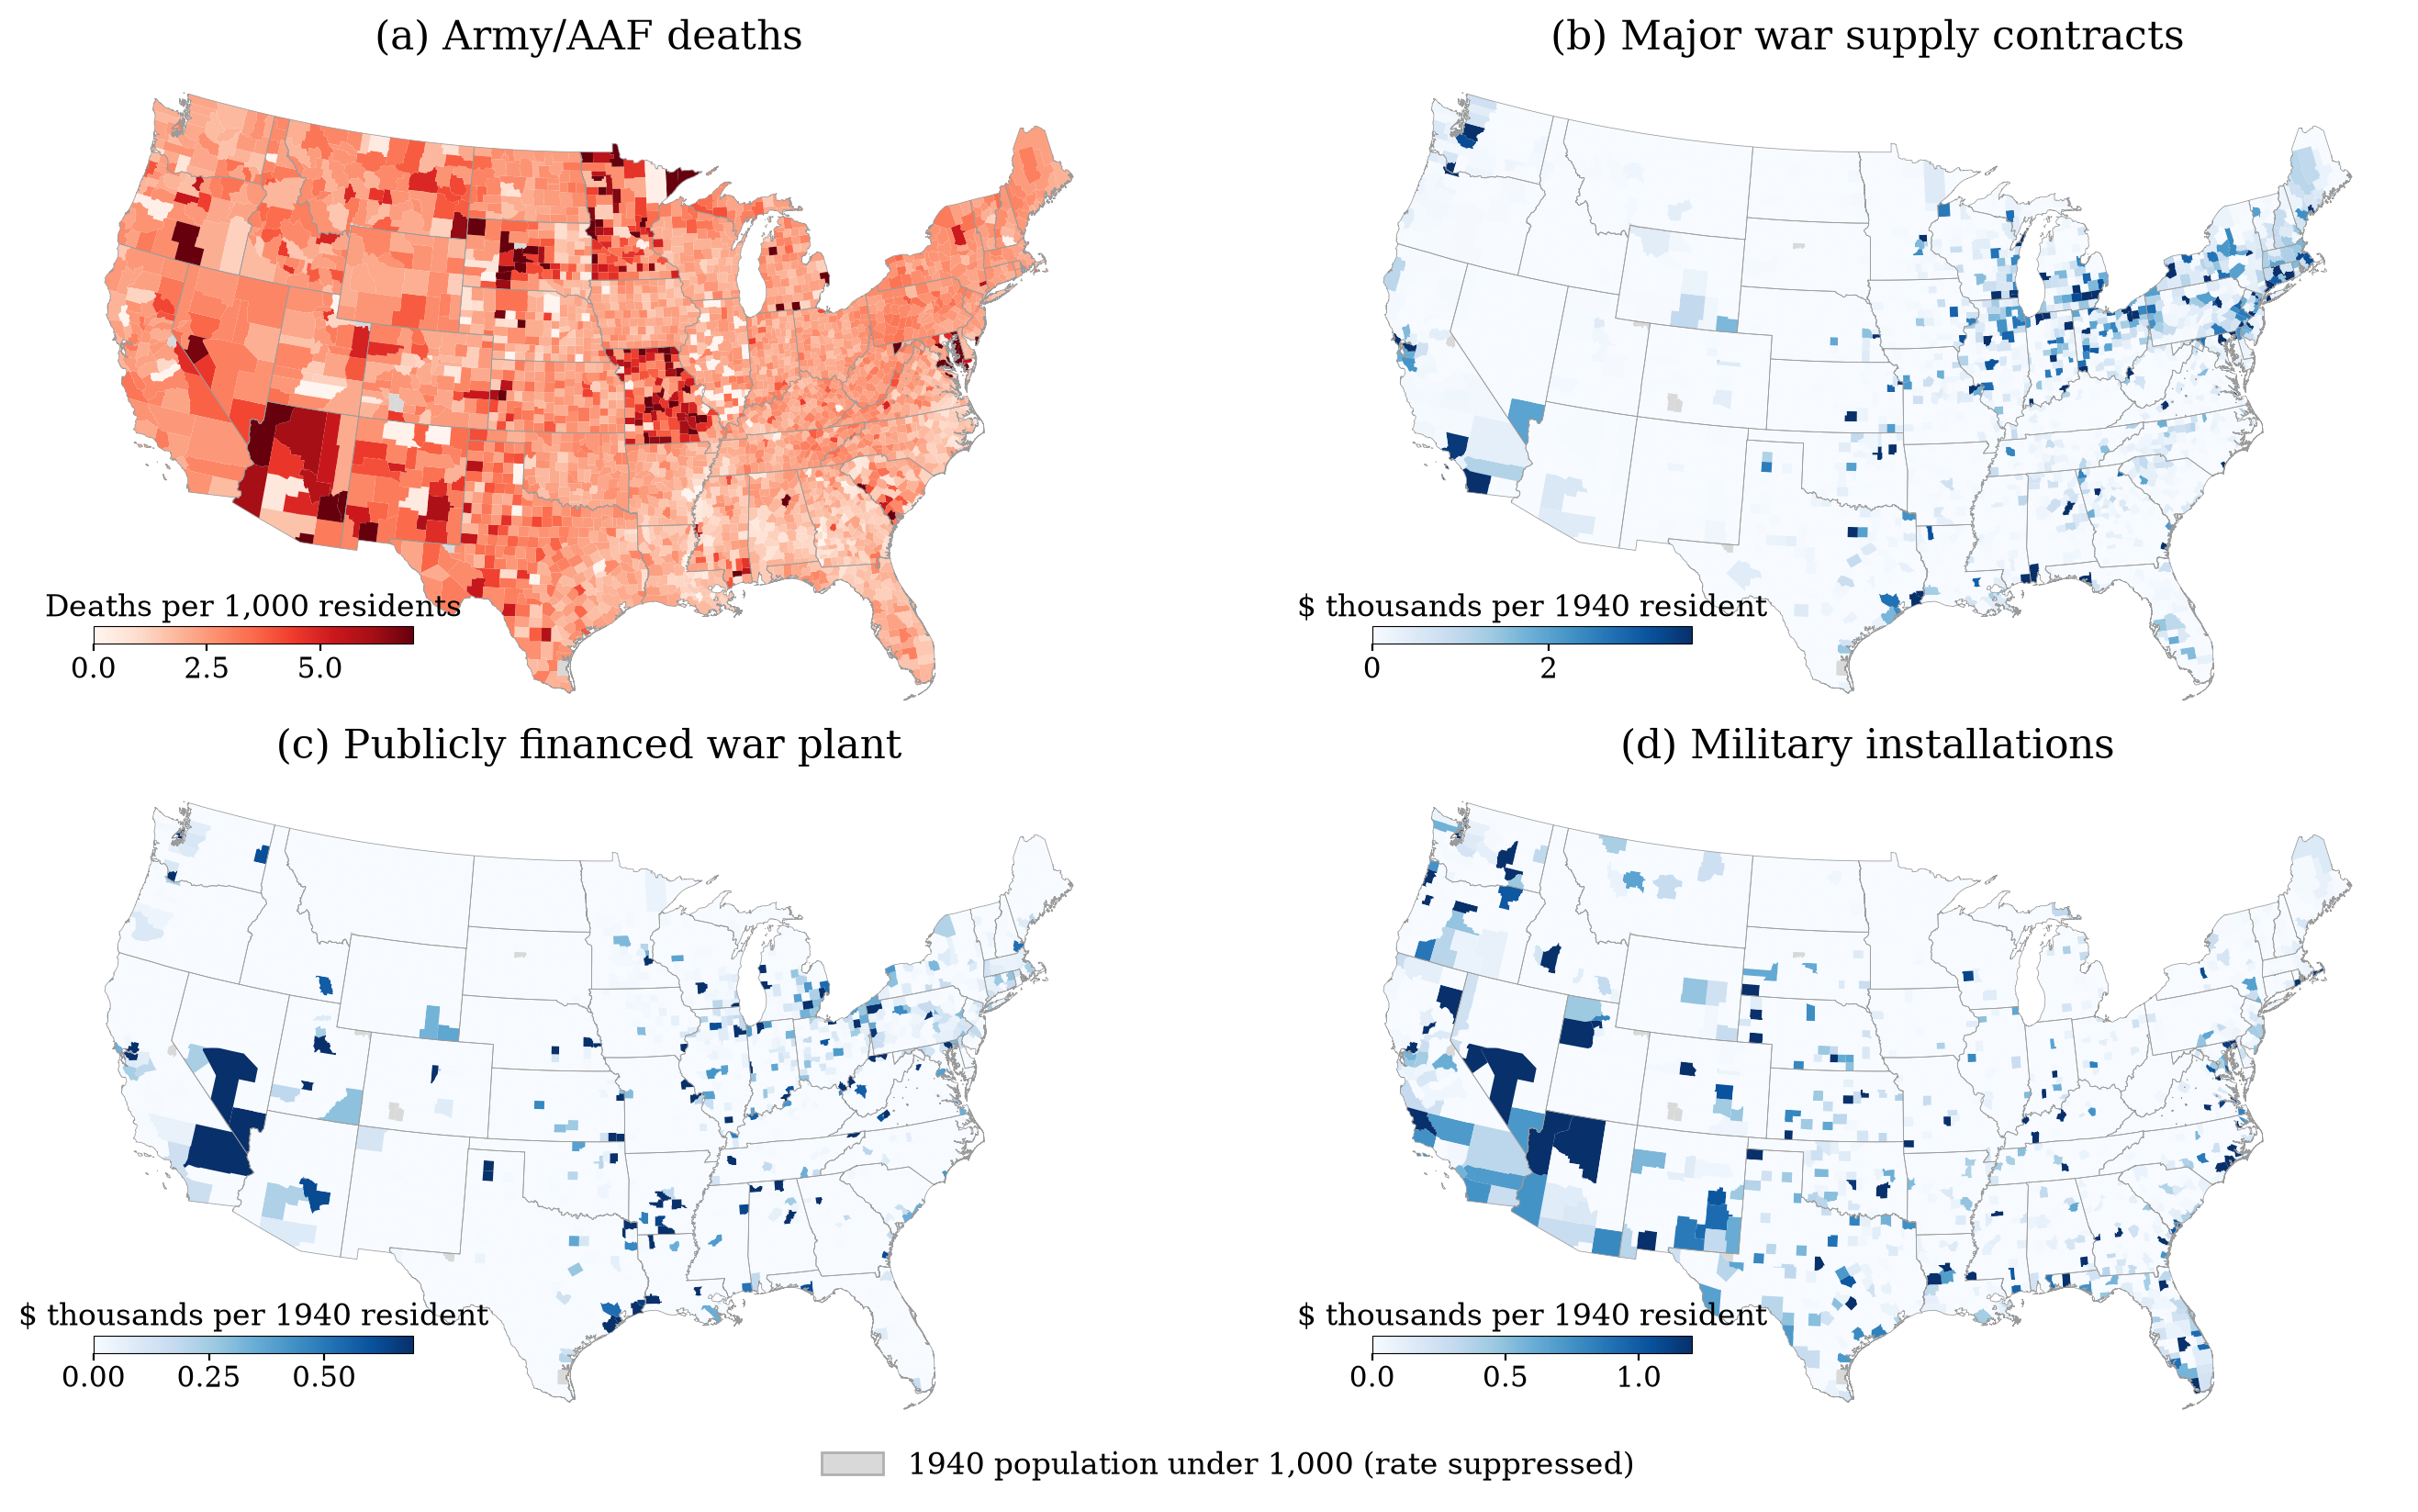
\includegraphics[width=\textwidth]{figures/fig_four_geographies.png}
\caption{The four wartime allocations on 1940 county boundaries}
\label{fig:four}
\vspace{2pt}
\begin{minipage}{\textwidth}\footnotesize \textit{Notes:} Panel (a) plots Army and Army Air Forces deaths per 1{,}000
1940 residents; panels (b), (c) and (d) plot major war supply contracts,
publicly financed industrial plant, and military installations, each in
thousands of current dollars per 1940 resident. Human loss is drawn on a red
ramp and federal dollars on a blue one, both running pale to dark, so that
counties receiving nothing recede rather than dominate the surface; the same
two hues form the poles of Figure \ref{fig:imbalance}. Note that the four
panels carry separate scales and are not directly comparable in magnitude: the
comparison of interest is the pattern of coverage, near-universal in panel (a)
and sparse in panels (b) through (d). Colour scales are trimmed at the 98th
percentile so that a small number of extreme counties do not compress the rest
of the distribution.\footnote{Trimming affects the display only. Every statistic reported in the text is computed on untrimmed data, with the two exceptions stated explicitly: the 99th-percentile cap on fatal burden before residualizing for Figure \ref{fig:imbalance}, and the suppression of counties below a thousand residents from both maps.} Counties with fewer than 1{,}000 residents in 1940 are
shown grey; a handful record impossible rates. Boundaries are the Newberry
Atlas of Historical County Boundaries as in effect 1 April 1940, with state
outlines drawn in grey; independent cities are merged into their surrounding
county. Albers equal-area projection.
\end{minipage}
\end{figure}

The coverage asymmetry is stark. Some 98.2 percent of counties recorded at least
one Army/AAF death, while 48.5 percent received any major contract:
\textbf{1{,}553 counties lost men and received no major war contract at all.} Table \ref{tab:top20} lists the twenty largest contract recipients. Concentration
is far higher for money than for loss: the twenty counties that lost the most men
hold 20.4 percent of the dead, while the twenty largest contract recipients hold
43.8 percent of the contract dollars; at a hundred counties the two figures are
40.7 and 81.3 percent. Loss was
distributed almost everywhere; investment was not.

The decisive statistic is what remains once county size is removed. Ranked across
counties, the correlation between fatal burden and war investment per resident is
$-0.026$ for contracts, $+0.013$ for industrial plant, and $-0.054$ for military
installations. Three separate allocation mechanisms, administered by different
agencies under different statutes, all produce a relationship with sacrifice
close to zero. Two of the three are not statistically distinguishable from zero
at all. The third is: at $n = 3{,}073$ the installation correlation of $-0.054$
has a confidence interval of $[-0.089, -0.018]$, which excludes zero
($p = 0.003$). It does so in the direction that makes the point sharper rather
than softer --- installations went, if anything, slightly \emph{away} from the
counties bearing the heaviest burden --- and it accounts for three-tenths of one
percent of the variance in installation spending.

The right way to read those three near-zeros is against the criteria the
procurement agencies were in fact selecting on, measured the same way, on the
same counties, in the same units. Table \ref{tab:criteria} does that. Per
resident, contract dollars correlate with the 1940 manufacturing share at
$+0.693$, with the 1940 urban share at $+0.648$, and with 1940 log population at
$+0.666$. Publicly financed plant and military installations load on the same
characteristics at $+0.23$ to $+0.51$. Against fatal burden all three read
$-0.026$, $+0.013$ and $-0.054$.

This is the paper's central quantitative statement, and it requires no
identifying assumption. The wartime allocation function put weights of roughly
$0.2$ to $0.7$ on prewar industrial capacity, urbanization and size, and a
weight of essentially zero on human loss. The near-zeros are precise rather
than underpowered: at $n = 3{,}073$ the standard error of a rank correlation is
$0.018$, so the confidence intervals exclude any association above $0.09$ in
absolute value, and a true correlation of the magnitude the agencies' own
criteria display would have been detected with near certainty.

\begin{table}[!htbp]
\centering
\caption{What the wartime allocation loaded on}
\label{tab:criteria}
\fittab{\begin{tabular}{lccc}
\toprule
& Contracts $W^C$ & War plant $W^F$ & Military $W^M$ \\
& (1) & (2) & (3) \\
\midrule
\multicolumn{4}{l}{\emph{Characteristics the procurement agencies selected on}} \\
\quad 1940 manufacturing share & +0.693 & +0.445 & +0.234 \\
\quad 1940 urban share & +0.648 & +0.507 & +0.398 \\
\quad 1940 log population & +0.666 & +0.514 & +0.328 \\
\multicolumn{4}{l}{\emph{Military sacrifice}} \\
\quad Fatal burden, per resident & -0.026 & +0.013 & -0.054 \\
\quad Fatal burden, per enlistee & -0.182 & -0.074 & -0.193 \\
\midrule
$N$, first four rows & 3,073 & 3,073 & 3,073 \\
$N$, per-enlistee row & 2,976 & 2,976 & 2,976 \\
\bottomrule
\end{tabular}}
\vspace{2pt}
\begin{minipage}{\textwidth}\footnotesize \textit{Notes:} Spearman rank
correlations between each wartime allocation, measured in dollars per 1940
resident, and the row characteristic. Fatal burden per resident is Army/AAF
deaths per 1{,}000 1940 residents; per enlistee is deaths per 1{,}000 Army/AAF
enlistees on the counties passing the validity screen of Section \ref{sec:data}. The
standard error of a rank correlation at $n = 3{,}073$ is $0.018$.
\end{minipage}
\end{table}

Conditioning on enlistment sharpens this rather than softening it. Using $B_i^{A}$
of equation (2)---deaths per thousand men actually enlisted, a national rate of
42.9 with a 90/10 county ratio of $3.58$---the correlations turn
\emph{negative}, at $-0.182$ for contracts, $-0.074$ for plant and $-0.193$ for
military installations against investment per resident (Table
\ref{tab:criteria}), and at $-0.157$, $-0.067$ and $-0.187$ if investment is put
on a per-enlistee footing as well.\footnote{The two sets differ only in the
denominator of the investment measure, not in the burden measure. Table
\ref{tab:criteria} reports the per-resident version so that every row of that
table shares one set of units.} Counties whose soldiers died at higher rates
received, if anything, less federal investment per soldier sent. Figure \ref{fig:imbalance} maps the
residualized difference between the two exposures, and shows that the counties
losing most relative to their investment are not concentrated in any one region
--- which is what an allocation indifferent to sacrifice, rather than hostile to
particular places, should look like.

\begin{table}[!htbp]
\centering
\caption{Did fatal burden predict federal war investment?}
\label{tab:allocation}
\fittab{\begin{tabular}{lccc}
\toprule
& Contracts $W^C$ & War plant $W^F$ & Military $W^M$ \\
& (1) & (2) & (3) \\
\midrule
$B_i$, state effects only & -0.0031 & -0.0019 & -0.0027$^{*}$ \\
 & (0.0032) & (0.0020) & (0.0015) \\
$B_i$, plus prewar controls & 0.0106$^{***}$ & 0.0071$^{***}$ & 0.0039$^{**}$ \\
 & (0.0019) & (0.0012) & (0.0018) \\
$B_i^{A}$, plus prewar controls & -0.0015 & 0.0006 & 0.0005 \\
 & (0.0020) & (0.0016) & (0.0020) \\
\midrule
State fixed effects & Yes & Yes & Yes \\
$N$ (rows 1--2; row 3) & \multicolumn{3}{c}{3,073; 2,976} \\
\bottomrule
\end{tabular}}
\vspace{2pt}
\begin{minipage}{\textwidth}\footnotesize \textit{Notes:} Dependent variables are inverse-hyperbolic-sine transforms of per-capita dollars; each cell is a separate regression. Prewar controls: 1940 log population, urban share, Black population share, manufacturing share, 1930--40 population growth, 1930 illiteracy and farm shares, and indicators for suppressed or imputed controls. All specifications carry state fixed effects. $B_i$ is deaths per 1{,}000 1940 residents; $B_i^{A}$ is deaths per 1{,}000 Army/AAF enlistees and is defined on the 2{,}976 counties passing the validity screen of Section \ref{sec:data}. Standard errors clustered on state in parentheses. $^{*}$, $^{**}$ and $^{***}$ denote significance at the 10, 5 and 1 percent levels.\end{minipage}
\end{table}

\begin{figure}[htbp]
\centering
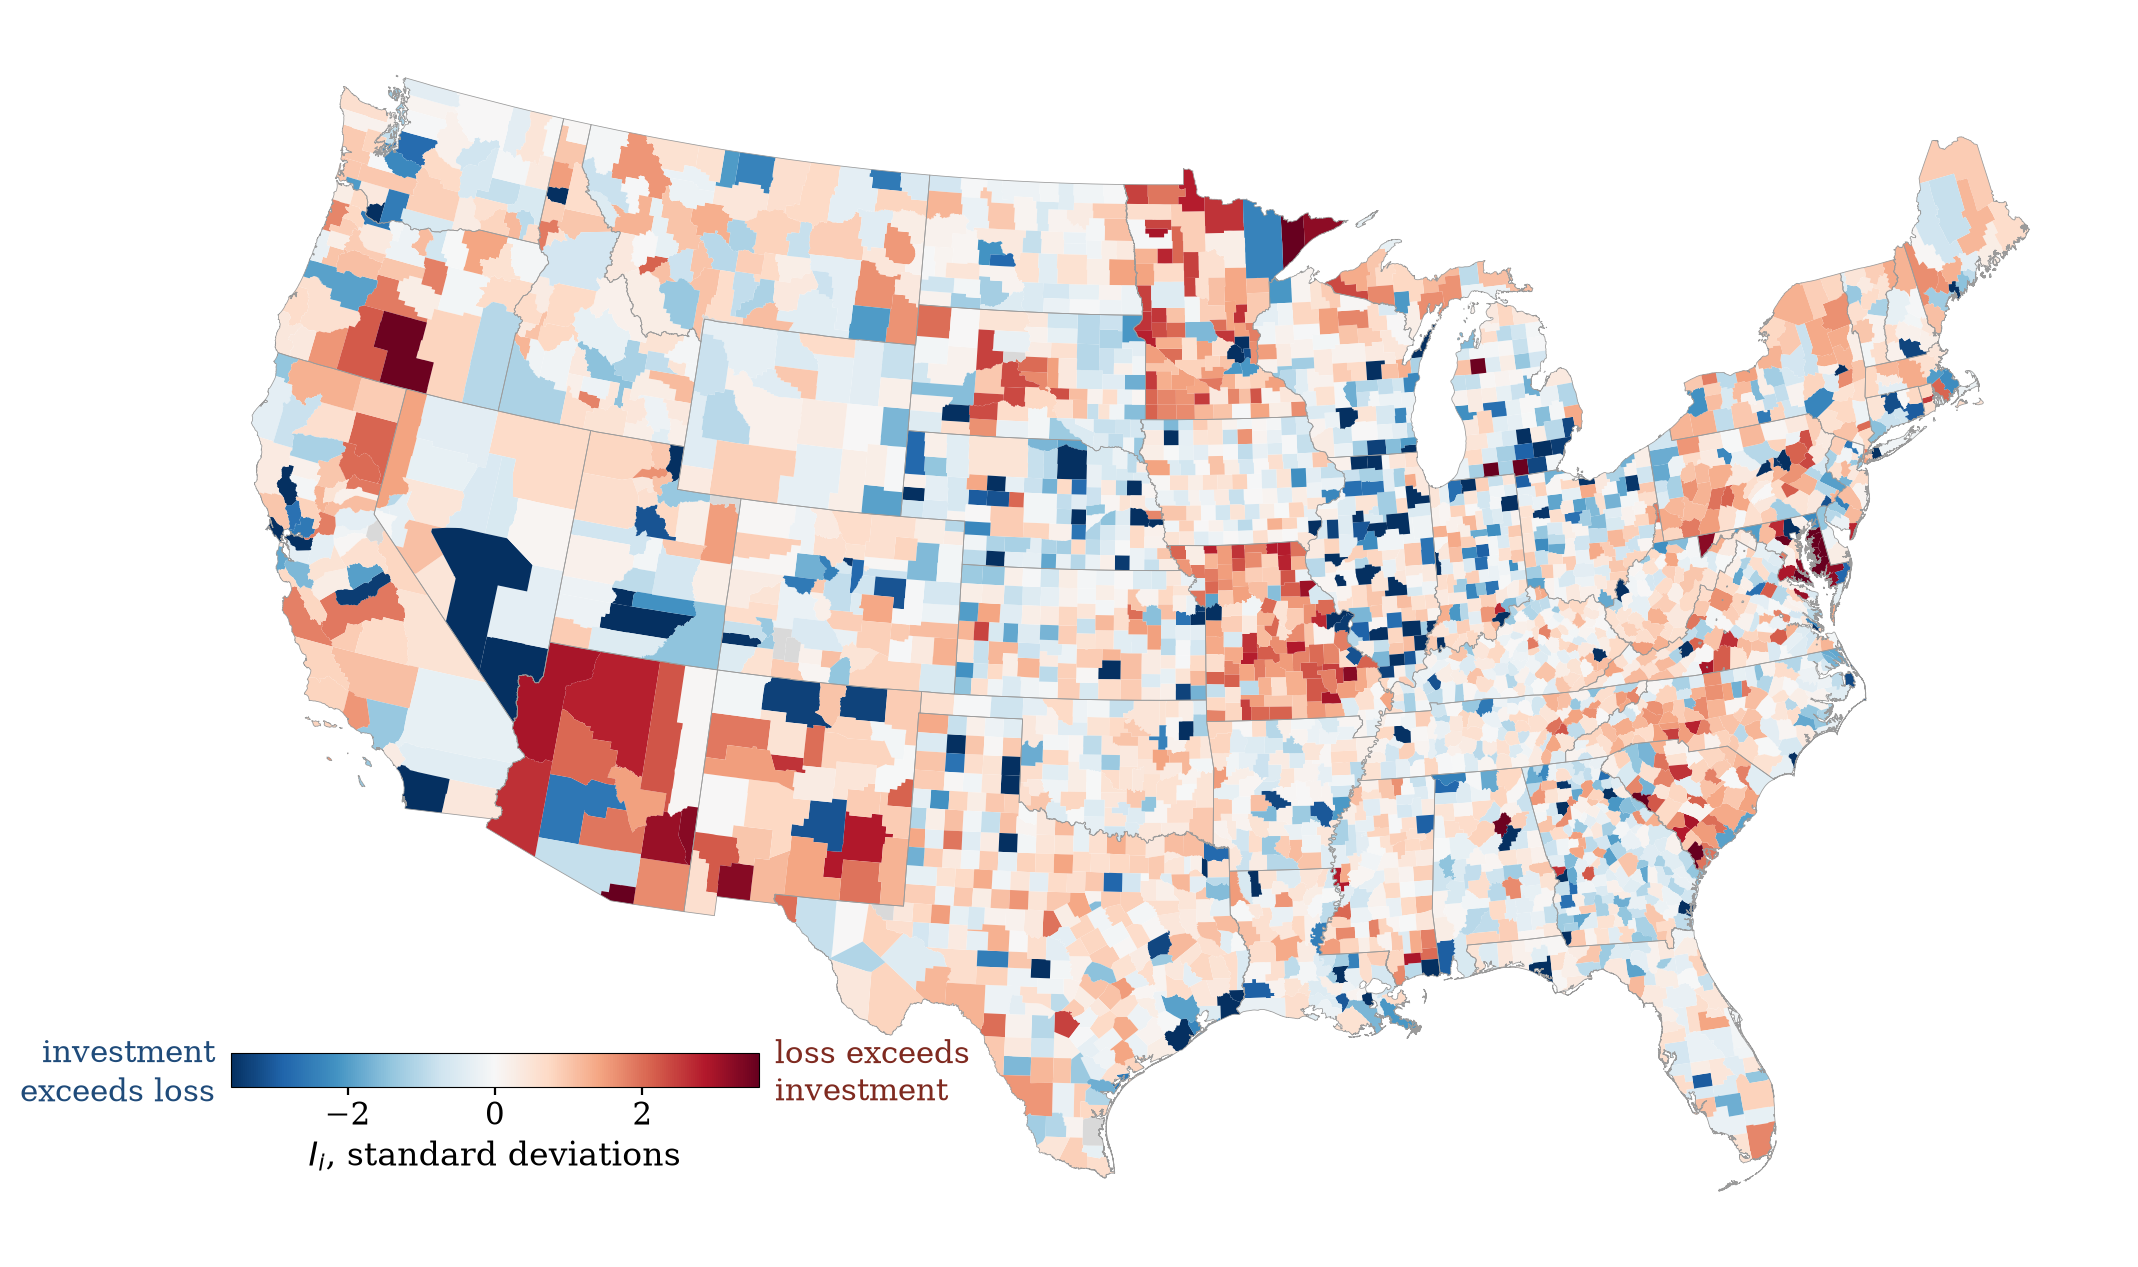
\includegraphics[width=\textwidth]{figures/fig_imbalance.png}
\caption{Conditional imbalance $I_i$ between sacrifice and investment}
\label{fig:imbalance}
\vspace{2pt}
\begin{minipage}{\textwidth}\footnotesize \textit{Notes:} Both exposures are residualized on 1940 log population, urban
share, Black population share, manufacturing share, and 1930--40 population
growth, then standardized; $I_i$ is the difference, reported in standard
deviations. Red counties lost more than their investment would predict, blue
counties the reverse; near-white counties are those where the two exposures
correspond. The scale is symmetric about zero and trimmed at the 97th
percentile of $|I_i|$. Fatal burden is capped at its 99th percentile before
residualizing so that transcription errors in a few very small counties cannot
dominate the surface. Boundaries and projection as in Figure \ref{fig:four}.
\end{minipage}
\end{figure}
 Table \ref{tab:allocation} regresses each
investment measure on fatal burden and reports three specifications, because the
answer depends on which burden measure is used and the difference is
instructive.

Without controls, fatal burden predicts none of the three; the only coefficient
that reaches even ten percent is a \emph{negative} one on military installations.
Adding the prewar vector turns all three positive and significant. This is worth
stating plainly rather than burying, because it is the one place in the paper
where a conditional association runs against the headline. What it does not do is
overturn it, for two reasons. The first is magnitude: moving a county from the
tenth to the ninetieth percentile of its death rate raises the inverse hyperbolic
sine of investment per resident by $0.024$ for contracts, $0.016$ for plant and
$0.009$ for military installations --- on the order of one to three percent of a
standard deviation of each, against distributions whose own tenth-to-ninetieth
range spans orders of magnitude. The second is that the result does not survive
the change of denominator. Under $B_i^{A}$, the per-enlistee measure this paper
argues is the right one for inference because it holds constant how many men a
county sent, no coefficient is distinguishable from zero ($p = 0.45$, $0.73$,
$0.81$). What conditioning on prewar structure recovers is a small positive
relationship between a county's civic death rate and its investment, and that
relationship disappears once the number of men exposed is held fixed.

The award dates make it possible to ask whether this is an average concealing a
change. Every one of the 190{,}693 contracts carries an award month, so the
allocation can be re-estimated separately for each year of the war, and
Table \ref{tab:byyear} does. It does not change. On the fixed set of 1{,}490 counties
that received a contract at some point, the rank correlation between per-capita
contract dollars and the 1940 manufacturing share is $0.497$ in 1940 and $0.588$
in 1945, moving non-monotonically in between.\footnote{The comparable rank
correlation computed across all 3{,}073 counties rises from $0.493$ to $0.653$,
but that movement is mostly coverage: 15.0 percent of counties received a
contract in 1940 against 40.1 percent in 1943, and a rank correlation over a
column that is 85 percent zeros is mechanically attenuated. The fixed-sample
figure is the one reported.} And the coefficient on fatal burden is
indistinguishable from zero in every single year under the per-enlistee measure
($p = 0.69$, $0.27$, $0.38$, $0.97$, $0.44$, $0.83$), on standard errors of
$0.0008$ to $0.0014$ against coefficients never exceeding $0.0012$ in absolute
value, so the annual zeros are as precise as the pooled one,
while under the per-resident measure it is in every year the same small positive
that the pooled specification of Table \ref{tab:allocation} reports. The war
state's indifference to sacrifice is not a property of the average. It held in
1940, when the allocation was small and highly selective, and it still held in
1945.

That $B_i^{A}$ is not a restatement of $B_i^{\mathrm{civic}}$ is worth establishing.
The two correlate at $0.628$, but they behave oppositely against mobilization
intensity: $B_i^{\mathrm{civic}}$ is nearly independent of the share of military-age
men who served ($\rho = +0.094$) whereas $B_i^{A}$ is strongly negatively related to
it ($\rho = -0.629$). Counties that mobilized more heavily lost a smaller fraction
of those they sent. A community-burden measure alone conflates sending many men with
losing many of those sent; separating them is what equation (2) is for.

\needlines{5}
\subsection{Postwar divergence}

Table \ref{tab:main} reports outcome regressions from 1940 through 1970 with prewar
controls, state fixed effects, and standard errors clustered on state. Three
patterns hold.

First, all three wartime allocations raised county population, and the military
coefficient is the largest of the three by 1970 ($+0.049$ against $+0.035$ for
contracts and $+0.020$ for plant). Population growth is therefore a poor proxy for
the kind of investment received.

Second, and centrally, the two forms of federal capital diverge sharply on
industrial structure. On the 1970 manufacturing share, contracts enter at $+0.33$
and industrial plant at $+0.29$, while military installations enter at $-0.59$.
The extensive margin is starker still: merely hosting a war plant is associated
with a manufacturing share $1.70$ points higher in 1970 ($p = 0.001$), merely
hosting a military installation with $3.72$ points lower ($p < 0.001$).

That contrast is real but it is not what it first appears, and the levels behind
the share say why. All three exposures raise total 1970 employment, and military
installations do so as strongly as contracts ($+0.042$ against $+0.041$, plant
$+0.021$). On manufacturing employment the ordering is different: contracts enter
at $+0.060$ and plant at $+0.027$, both at $p<0.001$, while installations enter at
$+0.014$ and reach only ten percent. The manufacturing share falls in installation
counties because their employment grew and their manufacturing did not grow with
it, not because manufacturing left. Federal money that arrived as productive plant
and federal money that arrived as payroll did not leave the same place behind ---
but the difference is what each of them built, not that one of them tore something
down. Section \ref{sec:milmatch} shows the same decomposition inside the matched
design.

Tenure is not a mirror of that result and should not be read as one. Military
investment enters at $-0.34$ on the 1970 ownership rate and is the only one of
the three distinguishable from zero; industrial plant enters at $+0.06$ and
contracts at $-0.05$, neither significant. Installations lowered ownership;
plants did nothing measurable to it. That asymmetry holds in the matched design
of Section \ref{sec:matched} as well, and it is the form the contrast actually
takes.

Table \ref{tab:interactions} reports the interactions of
equation~\eqref{eq:baseline}. Three of the four pairs are null. The exception is
the 1970 manufacturing share, where $\theta_C = +0.0115$ ($p < 0.001$) and
$\theta_F = +0.0036$ ($p = 0.10$): procurement's association with postwar
industrial structure was larger in counties whose soldiers died at higher rates.
The magnitude is not trivial --- moving across the tenth-to-ninetieth range of
$B_i^{A}$ among counties that received a contract adds roughly $0.6$ to a main
effect of $0.33$ --- and it is the one
place where fatal burden enters an outcome equation with force. It does not bear
on the allocation result, which is about where investment went rather than what
it did, and I report it as an association without a mechanism.

Third, fatal burden predicts essentially nothing on its own. The one coefficient in
Table \ref{tab:main} that reaches significance is the 1950 population term, and
it is negligible: $+0.0009$ log points per additional death per thousand
residents, so the entire tenth-to-ninetieth range of the county death rate moves
1950 population by under half a percent.

\begin{table}[htbp]
\centering
\caption{Wartime exposure and postwar county outcomes, 1950--1970}
\label{tab:main}
\fittab{\begin{tabular}{lccccccc}
\toprule
& (1) & (2) & (3) & (4) & (5) & (6) & (7) \\
& Log pop. & Log pop. & Mfg.\ share & Mfg.\ share & Log income & Log income & Own rate \\
& 1950 & 1970 & 1960 & 1970 & 1950 & 1970 & 1970 \\
\midrule
Contracts $W^C_i$ & 0.0118$^{***}$ & 0.0346$^{***}$ & 0.4594$^{***}$ & 0.3325$^{***}$ & 0.0125$^{***}$ & 0.0148$^{***}$ & -0.0483 \\
 & (0.0015) & (0.0035) & (0.0833) & (0.1016) & (0.0024) & (0.0016) & (0.0902) \\
War plant $W^F_i$ & 0.0103$^{***}$ & 0.0197$^{***}$ & 0.4165$^{***}$ & 0.2851$^{***}$ & 0.0087$^{**}$ & 0.0101$^{***}$ & 0.0562 \\
 & (0.0025) & (0.0046) & (0.0752) & (0.0829) & (0.0034) & (0.0025) & (0.0861) \\
Military $W^M_i$ & 0.0175$^{***}$ & 0.0493$^{***}$ & -0.4558$^{***}$ & -0.5945$^{***}$ & 0.0121$^{***}$ & 0.0086$^{***}$ & -0.3360$^{***}$ \\
 & (0.0017) & (0.0047) & (0.0835) & (0.1108) & (0.0027) & (0.0017) & (0.0547) \\
Fatal burden $B_i$ & 0.0009$^{***}$ & -0.0023 & -0.0968 & -0.0798 & -0.0001 & -0.0013 & -0.1335 \\
 & (0.0002) & (0.0026) & (0.0650) & (0.0961) & (0.0023) & (0.0010) & (0.1164) \\
\midrule
Prewar controls & Yes & Yes & Yes & Yes & Yes & Yes & Yes \\
State fixed effects & Yes & Yes & Yes & Yes & Yes & Yes & Yes \\
$N$ & 3,072 & 3,065 & 3,071 & 3,066 & 3,010 & 3,066 & 3,066 \\
$R^2$ & 0.984 & 0.929 & 0.745 & 0.697 & 0.774 & 0.641 & 0.472 \\
\bottomrule
\end{tabular}}
\vspace{2pt}
\begin{minipage}{\textwidth}\footnotesize \textit{Notes:} All specifications include the full prewar control set and state fixed effects. Standard errors clustered on state in parentheses. Income outcomes are logged. Coefficients are conditional associations, not causal effects; see the pre-trend evidence in Table \ref{tab:pretrends}. $^{*}$, $^{**}$ and $^{***}$ denote significance at the 10, 5 and 1 percent levels.\end{minipage}
\end{table}
 Across population, manufacturing,
income, and homeownership, and under four alternative denominators---residents,
adult males, men in the labor force, and battle deaths only---no specification
yields a coefficient distinguishable from zero at conventional levels
(Table \ref{tab:burden}). What a county
gave the war did not shape what it kept from it.

\needlines{5}
\subsection{Whose sons, and in which branch}

The enlistment file records race, education, birth year and enlistment source
for every soldier, and the Army General Classification Test score for 5.4 percent
of them, which makes it possible to ask whether county differences in fatality
rates reflect differences in risk or differences in who was sent. The test-score
term should be read with that coverage in mind: a county's mean rests on roughly
one enlistee in twenty, and 139 counties carry no scored record at all and take
the sample median. Restricting to the 2{,}966 counties with
at least a hundred enlistees --- covering 7.17 million enlistees and 288{,}059
deaths --- and regressing the county fatality rate on the composition of its
soldiers gives $R^2 = 0.177$.

The coefficients are informative in themselves. A larger volunteer share raises
the county fatality rate sharply, a larger share of Black enlistees lowers it,
and higher average education and test scores raise it. All four run through
assignment to branch: volunteers and high-scoring men were channeled toward the
Army Air Forces and the airborne divisions, while Black soldiers were
concentrated in service and supply units under the segregated manpower policy of
the period, a pattern consistent with the occupational evidence in
\textcite{ferrara2022}. A county's fatality rate was therefore not only a
function of how many men it sent but of which parts of the Army they entered.

Composition accounts for 9.3 percent of the cross-county standard deviation in
fatality rates, so the great majority of the variation survives adjustment.
Residualizing the rate on composition does not weaken the paper's central
result; it strengthens it. The rank correlation between composition-adjusted
fatality risk and per-capita investment is $-0.182$ for contracts, $-0.119$ for
industrial plant, and $-0.083$ for military installations. For contracts and
plant the adjustment makes the correlation more negative, not less
($-0.170$ and $-0.070$ before it); for military installations it moves the other
way, from $-0.178$ to $-0.083$.\footnote{The unadjusted figures here differ
slightly from the per-enlistee row of Table \ref{tab:criteria} because this
exercise runs on the 2{,}966 counties with at least a hundred enlistees and uses
the fatality rate built from the DS2 decode, which is the universe the
individual composition variables are defined on.} All three remain negative under either
treatment. Counties whose men faced higher risk conditional on who they sent
received no more federal investment, and by these estimates slightly less.

\needlines{5}
\subsection{What the estimates can and cannot support}

Two results discipline the interpretation. Spatial standard errors computed with a
Conley kernel at 200 kilometers leave every sign and significance level in place,
so the findings are not an artifact of treating neighboring counties as
independent (Table \ref{tab:conley})\footnote{Two hundred kilometers is roughly
the radius within which a county's labor market and its wartime procurement
neighbors are likely to overlap. Six of the eight spatial standard errors are
tighter than the state-clustered ones, though one of the six only in the fifth
decimal; the two that are not are contracts on 1970
population, where the Conley error is 0.0042 against 0.0034 and the $t$ statistic
is still 8.25, and war plant on the 1970 manufacturing share, at 0.0873 against
0.0829 and $t = 3.26$. The state-clustered errors are reported throughout because
they are the more conservative of the two in six of eight cases and the exceptions
change nothing.}; and dropping the twenty largest contract
recipients changes no sign or significance and moves no coefficient by more than
five percent of its own value (Table \ref{tab:droptop}), so
they are not driven by a handful of arsenal counties.

A source limitation should be recorded. The Army/AAF honor list is not complete
at county level: matched to the 1940 census, 56 of 3{,}073 counties carry no
recorded death, and they are concentrated in Illinois, where 80 of 102 counties
appear and the implied death rate is 1.90 per thousand residents against a
national 2.26. Nebraska is next with seven. Independent cities are
split inconsistently between city and surrounding county in Maryland, Missouri, and
Virginia. Excluding Illinois entirely leaves every sign and every
significance level in Table \ref{tab:main} intact. The largest movement is
$+0.018$, on the contract coefficient for the 1960 manufacturing share
($0.459$ to $0.477$), which is about a fifth of that coefficient's standard
error; $\mathcal{A}$ shifts from $0.466$ to $0.454$. The state matters enough to
be worth reporting and not enough to carry a result.
The cross-state variation that remains is substantially real rather than
artifactual: New Mexico's rate of 3.61 per thousand, the highest of any state,
reflects the destruction of the 200th Coast Artillery on Bataan.\footnote{The 200th Coast Artillery (Anti-Aircraft) was a New Mexico National Guard regiment federalized in 1941 and sent to the Philippines. Roughly half its men died in captivity after the surrender of Bataan, and the regiment drew disproportionately from a small number of New Mexico counties. This is the clearest illustration in the data of the paper's point about branch and unit assignment: a county's fatality rate depended on which formation its men entered, not only on how many it sent.}

Against this, a placebo test is partly unfavorable. Wartime exposure was assigned
between 1940 and 1945 and so should not predict earlier outcomes, yet contracts and
military installations both predict 1930--40 population growth, and both predict
the prewar manufacturing share --- contracts positively and installations
negatively (Table \ref{tab:pretrends}). Federal investment went
disproportionately to counties already growing. Contract dollars went to counties
already industrial; installations went away from them, which is the same
divergence Section \ref{sec:threealloc} reports and not a second confound.

Carrying the same test back one further decade bounds what that means. Against
1920--30 population growth --- before the Depression as well as before the war ---
no exposure predicts anything: contracts enter at $+0.0004$ ($p = 0.85$), plant at
$+0.0044$ ($p = 0.26$), installations at $+0.0008$ ($p = 0.85$), and fatal burden
at $-0.0004$ ($p = 0.81$), on the 3{,}041 counties whose 1920 population can be
matched.\footnote{From Haines part 24. The match totals 105.7 million residents
against a 1920 continental census of 105.7 million; the thirty-one counties that
fail to match were created after 1920, and one further county lacks a usable 1920
figure. Together they hold 0.14 percent of 1940 population.}
The counties that later received war investment were not on a different
trajectory in the 1920s. What Table \ref{tab:pretrends} records is a
Depression-decade divergence, which is a narrower and more tractable problem than
a long-running one, though it remains a reason to read Table \ref{tab:main} as
conditional association. Fatal burden runs the other way: casualty-heavy counties were already
losing population before the war. The estimates in Table \ref{tab:main} are
therefore reported as conditional associations on a rich prewar control set, not as
causal effects. The industrial-plant pre-trend is the mildest of the three, which is
a point in favor of the publicly financed plant design of \textcite{garin2025};
Section \ref{sec:matched} builds a quasi-experimental treatment on $G_i$ and
reports it.

One further hypothesis was tested and rejected. If loss and investment diverged, a
natural conjecture is that casualty-heavy counties received bases rather than
plants---payroll rather than productive capital. The raw pattern is suggestive: among
counties receiving one type only, 34.2 percent of the lowest-burden quartile
received a plant against 54.9 percent of the highest. The association does not
survive prewar controls and state fixed effects: the coefficient on fatal burden
falls to $0.0002$ with a standard error of $0.0029$ and $p = 0.95$, and it is
reported here as a null. The
divergence is not that sacrifice bought the wrong kind of investment. It is that
sacrifice bought no particular kind at all.

\needlines{5}
\subsection{A matched comparison of large public plants}
\label{sec:matched}

The instrument fails because prewar industrial capacity predicts both treatment
and outcome. A design that does not require an instrument can still succeed if
it compares treated counties to counties that look like them on exactly that
dimension. This is the strategy of \textcite{garin2025}, and I implement it
here.

\emph{Treatment.} A county is treated if it received at least one plant that
was publicly financed (private share of structure spending at most five
percent), newly built (structures above forty percent of plant cost), and large
(cost of at least \$10 million). The facilities report marks new construction with an explicit
\texttt{New Plant} designation printed beneath a facility's location; combined
with the structure-share rule this yields 226 qualifying plants worth
\$8.61 billion, of which 214 resolve to a county. Those 214 are worth
\$8.08 billion, are spread across 164 counties after the independent-city merge,
and carry 93.9 percent of the qualifying dollars. Measured against the base
\textcite{garin2025} report on --- spending on all newly built wartime plants,
publicly and privately financed, which the facilities volume puts at
\$11.94 billion --- the 226 capture 72.1 percent, against roughly 70 percent for
their 353-plant definition. The two selections therefore cover the same ground;
the count differs because the unit of record here is a
cost line while theirs is a deduplicated plant identifier.

\emph{Sample.} The hundred largest manufacturing counties of 1940 are dropped.
These are the places whose selection into treatment is least comparable to
anything else, and retaining them means estimating a contrast between Detroit
and rural Georgia.\footnote{The restriction also removes the region of the propensity distribution where common support is thinnest. It is imposed on the estimation sample throughout rather than varied as a robustness check, so no result in the paper rests on a comparison involving the largest prewar manufacturing centers.} After this restriction the sample is 2{,}973 counties, of
which 118 are treated.

\emph{Matching.} A propensity score is estimated on the prewar vector --- 1940
log population, urban share, Black population share, manufacturing share,
1930--40 population growth, 1930 illiteracy and farm shares, and latitude and
longitude, with squared terms --- and treated counties are matched to at most
three controls within a caliper of 0.2 standard deviations, on common support.\footnote{The caliper follows the convention of one-fifth of a standard deviation of the propensity score. Table \ref{tab:matchedrobust} varies it from 0.1 to 0.5 and varies the number of matched controls from one to five; the 1970 population coefficient stays within $0.193$ to $0.211$ across all five.}
115 of 118 treated counties match to distinct control counties.

\emph{Balance.} Table \ref{tab:balance} reports standardized mean differences.
Before matching, seven of the nine covariates exceed the conventional
0.10 threshold, and log population differs by 1.45 standard deviations. After
matching, \textbf{only two still do}. The two that do are
latitude ($-0.124$), a geographic coordinate rather than a measure of economic
structure, and the 1940 Black population share ($0.107$), which sits just past
the threshold and enters the outcome regressions as a control in any case. On
prewar population, urbanization, industrial structure and growth --- the
dimensions on which selection into treatment actually operated --- the treated
and control groups are balanced to within $0.10$ standard deviations.

\emph{Estimates.} Table \ref{tab:matched} reports the results. Receiving a large
new publicly financed plant is associated with a 1970 population 23.3 percent
higher, a manufacturing share 3.34 points higher, and family income 7.3 percent
higher, all relative to matched controls and all significant at the one percent
level. Homeownership is the exception and is reported as a null: the point
estimate is $+0.94$ points with a standard error of $0.61$, which does not reach
significance at any conventional level. Inverse-probability weighting on common
support gives the same signs throughout and larger magnitudes for population,
manufacturing and income.

\begin{table}[htbp]
\centering
\caption{Effect of a large new publicly financed wartime plant, matched comparison}
\label{tab:matched}
\fittab{\begin{tabular}{lrrrrr}
\toprule
Outcome & Raw difference & Matched & (SE) & IPW & $N$ \\
\midrule
log population 1970 & 1.3970 & 0.2092$^{***}$ & (0.0605) & 0.3041 & 364 \\
manufacturing share 1970 & 3.9528 & 3.3378$^{***}$ & (0.8458) & 3.6874 & 364 \\
log family income 1970 & 0.2201 & 0.0704$^{***}$ & (0.0194) & 0.1115 & 364 \\
homeownership 1970 & -1.6707 & 0.9416 & (0.6117) & 0.5376 & 364 \\
log family income 1950 & 0.2865 & 0.0647$^{***}$ & (0.0189) & 0.1011 & 364 \\
manufacturing share 1960 & 6.4296 & 3.2824$^{***}$ & (0.8310) & 4.1448 & 364 \\
log total employment 1970 & 1.4425 & 0.2228$^{***}$ & (0.0646) & 0.3044 & 364 \\
log manufacturing employment 1970 & 1.7126 & 0.3878$^{***}$ & (0.0854) & 0.5126 & 364 \\
\bottomrule
\end{tabular}}
\vspace{2pt}
\begin{minipage}{\textwidth}\footnotesize
\textit{Notes:} 115 treated counties matched to 249 distinct controls within a
0.2 standard-deviation caliper on the propensity score, excluding the 100
largest manufacturing counties of 1940. Matching is three-to-one with
replacement; $N$ is the number of distinct counties on the matched sample. Matched estimates are weighted least squares on the matched
sample with the full prewar covariate vector; IPW is inverse-probability
weighting on common support. Standard errors clustered on state.
Balance in Table \ref{tab:balance}; placebo tests in Table
\ref{tab:matchedplacebo}; robustness in Table \ref{tab:matchedrobust}. $^{*}$, $^{**}$ and $^{***}$ denote significance at the 10, 5 and 1 percent levels.
\end{minipage}
\end{table}

\emph{Placebo.} Table \ref{tab:matchedplacebo} applies the same estimator to
outcomes determined before the plants were sited. On the two that describe prewar
economic structure treatment predicts nothing: 1930--40 population growth
($p = 0.66$) and the 1940 manufacturing share ($p = 0.81$) are indistinguishable
between treated and matched control counties. This is the test the instrument
failed, and on those dimensions the matched design passes it.

The third is weaker and deserves saying plainly. Treated counties had a 1940
homeownership rate $1.27$ points above their matched controls, at $p = 0.11$ ---
short of significance at five percent, but not comfortably so, and larger in
magnitude than the $+0.94$ the same design estimates for 1970. A pre-treatment
coefficient that exceeds the post-treatment one is not evidence of an effect; it
is a reason to treat tenure as the dimension this design does not identify. That
is the conclusion the paper reaches below on independent grounds, and the placebo
is why it is reached rather than assumed.

\emph{What survives the hardest comparison.} Table \ref{tab:matchedrobust}
varies the matching parameters and the sample. Results are stable across one-,
three- and five-nearest-neighbor matching, across calipers of 0.1 to 0.5
standard deviations, and across restrictions of the sample to counties above
ten thousand residents or with any 1940 manufacturing employment; the 1970
population coefficient stays within $0.193$ and $0.217$ across all seven.
The demanding test is the last panel, which compares treated counties only to
their own untreated neighbors. The control pool is restricted to the 475
untreated counties that directly border a treated one --- places sharing a labor
market, a climate, and a state --- and 111 of the 118 treated counties find a
match inside it. There the population effect ($+0.180$, $p = 0.002$), the manufacturing
effect ($+1.63$, $p = 0.022$) and the income effect ($+0.045$, $p = 0.012$) all
survive, at magnitudes between roughly half and the whole of the matched-control
estimate. Homeownership is again indistinguishable from zero ($+0.40$,
$p = 0.48$).

One quantity should be attached to that claim before it is made. Both designs
are selection on observables, and Section \ref{sec:iv} argues at length that
prewar industrial capacity reaches 1970 outcomes by routes that do not pass
through wartime production. \textcite{oster2019} gives the natural bound: how
strong would selection on unobservables have to be, relative to selection on the
prewar vector already in the model, to drive each estimate to zero? Table
\ref{tab:oster} reports it, and the answer separates the two designs.

The plant estimates are the more fragile. At Oster's own $R^2_{\max}=1.3R^2$,
$\delta$ is $3.50$ for the manufacturing share and $1.51$ for family income,
both above the conventional threshold of one --- but $0.98$ for population and
$0.86$ for manufacturing employment, both just below it. Under the stricter
$R^2_{\max}=1$ only the manufacturing share survives. The table shows why: the
raw plant-county gap in 1970 log population is $1.78$, and the prewar vector
alone takes it to $0.23$. When the observables already account for that much of
a raw association, Oster's arithmetic says unobservables of comparable strength
would account for the rest. This is the same fact Section \ref{sec:iv} argues
from a different direction, and it is a real qualification rather than a
technicality.

The military estimates are the more robust, and two of them robust in the
stronger sense. For population ($-19.9$) and family income ($-26.4$) $\delta$ is
negative, because adding the prewar vector moves those coefficients \emph{away}
from zero rather than toward it: observed selection runs against the estimated
effect, so unobserved selection would have to be correlated in the opposite
direction to overturn it. For the manufacturing share and for homeownership
$\delta$ is $4.70$ and $23.25$, and remains above one at $R^2_{\max}=1$ ($1.66$
and $4.32$).

I therefore claim causal identification unevenly. The plant effect on the
manufacturing share is robust on this test at either $R^2_{\max}$; the effect on
family income is robust at Oster's and not at the stricter bound; the effects on
population and on manufacturing employment sit at the threshold, and I report
them as estimates that a referee is entitled to discount. Large publicly
financed wartime plants raised the population, the manufacturing employment, and
the family income of the counties that received them, and those effects persist
to 1970 and survive comparison against immediate neighbors --- but only the
industrial composition among them is insulated from a confounder as strong as
prewar industrial capacity itself. They did not measurably change the rate at
which those counties' residents owned their homes, against either comparison
group.

This matters for the paper's central question. The counties that received
durable public capital did acquire lasting economic advantages --- and Section
\ref{sec:results} shows that which counties those were had essentially nothing
to do with which counties bore the war's human cost.

\needlines{5}
\subsection{The same design applied to military installations}
\label{sec:milmatch}

\textcite{garin2025} establish the long-run effect of large publicly financed
industrial plants. No comparable estimate exists for the war's other great
federal capital allocation. Section \ref{sec:results} showed that industrial
plant and military installations occupy weakly related geographies and are
associated with opposite postwar structures. That association is what this
section tests.

Treatment is membership in the top decile of per-capita military facility
spending in the 1947 County Data Book, taken among the counties that received any
such spending and within the estimation sample. Fifty-six counties clear the
threshold; two of them also received a large public plant and are dropped so the
two treatments do not contaminate one another, leaving the 54 the design
actually studies. Those 54 hold \$2.01 billion, 25 percent of the military
facility dollars in the sample they are drawn from and 20 percent of the
national total. Matching proceeds exactly as in
Section \ref{sec:matched}: 52 of the 54 match to 152 controls, and
the treated counties are spread across 27 states with at most four in any one,
imbalance falls from eight of nine covariates to one, and all three placebo
tests are clean --- 1930--40 population growth ($p = 0.66$), the 1940
manufacturing share ($p = 0.63$), and the 1940 home-ownership rate
($+0.53$ points, $p = 0.70$), which is the pre-treatment outcome the design's
headline result most needs (Table \ref{tab:milplacebo}).

Table \ref{tab:twotreatments} sets the two treatments side by side, and the
contrast is the paper's sharpest result. A military installation raised county
population by 1970 far more than a war plant did --- 55 log points against 21 ---
while \emph{reducing} the manufacturing share by 4.72 points where the plant
raised it by 3.34. Family income rose under both. On homeownership the two
designs do not mirror each other: the installation effect is $-7.49$ points and
the plant effect is a null, so the tenure result belongs to installations alone.

The manufacturing rows carry a distinction the share alone cannot make. A share
falls either because its numerator shrinks or because its denominator grows, and
those are different histories. The employment levels separate them, and the
answer is the second. Total 1970 employment rose under both treatments, by 41 log
points for an installation and 22 for a plant. Manufacturing employment rose by
39 log points under a plant ($p < 0.001$) and by 22 under an installation, where
it is imprecise rather than zero ($p = 0.10$). Installations did not
deindustrialize the counties that received them; they grew everything else around
a manufacturing base that did not move, and the falling share is that arithmetic.
The plant is the opposite case: its manufacturing employment grew faster than its
employment as a whole, which is why the share rose. So the two treatments do not
have opposite effects on manufacturing. One of them has an effect on
manufacturing and the other has an effect on everything else --- which is the
sharper statement, and the one the county panel can actually support.

\begin{table}[htbp]
\centering
\caption{Two forms of federal capital, matched designs}
\label{tab:twotreatments}
\fittab{\begin{tabular}{lrrrr}
\toprule
& \multicolumn{2}{c}{Large public plant} & \multicolumn{2}{c}{Military installation} \\
\cmidrule(lr){2-3}\cmidrule(lr){4-5}
Outcome, 1970 & Effect & (SE) & Effect & (SE) \\
\midrule
Log population 1970 & 0.2092$^{***}$ & (0.0605) & 0.5509$^{***}$ & (0.0792) \\
Log total employment 1970 & 0.2228$^{***}$ & (0.0646) & 0.4141$^{***}$ & (0.0854) \\
Log manufacturing employment 1970 & 0.3878$^{***}$ & (0.0854) & 0.2151 & (0.1318) \\
\addlinespace
Manufacturing share 1970 & 3.3378$^{***}$ & (0.8458) & -4.7201$^{***}$ & (1.3957) \\
Log family income 1970 & 0.0704$^{***}$ & (0.0194) & 0.1051$^{***}$ & (0.0255) \\
Homeownership 1970 & 0.9416 & (0.6117) & -7.4890$^{***}$ & (1.1235) \\
\midrule
Treated counties & 115 & & 52 & \\
Covariates imbalanced & 2 of 9 & & 1 of 9 & \\
\bottomrule
\end{tabular}}
\vspace{2pt}
\begin{minipage}{\textwidth}\footnotesize
\textit{Notes:} Each column pair is a separate matched design estimated on its own propensity
score, excluding the 100 largest manufacturing counties of 1940 and, for the
military design, counties receiving both treatments. Weighted least squares on
the matched sample with the full prewar covariate vector; standard errors
clustered on state, 44 state clusters for the plant design and 40 for the
military design, of which 38 and 27 respectively carry a treated county. Because
27 is thin for cluster-robust inference, the military estimates are reported
alongside the randomization inference of Table \ref{tab:milrobust}, which
assumes nothing about the cluster structure. The first three rows are in logs; manufacturing employment
is the 1970 manufacturing share applied to 1970 total employment, and the two
employment rows decompose the share row beneath them rather than adding a
finding to it. Placebo tests in Tables \ref{tab:matchedplacebo} and
\ref{tab:milplacebo}.
\end{minipage}
\end{table}

Two forms of federal capital, arriving in the same years under the same war,
therefore left different places behind. The installation counties grew faster
and their residents earned more, but they grew in everything except
manufacturing and they did so with markedly lower rates of ownership. The plant
counties grew less, industrialized, and left tenure where they found it.\footnote{The plant
coefficient on 1970 homeownership is $+0.94$ points against matched controls
($p = 0.12$), $+0.40$ against untreated neighbors ($p = 0.48$), and
indistinguishable from zero in the continuous specification of
Table \ref{tab:main}. The installation coefficient is $-7.49$ points and
survives every specification tried. The asymmetry is stated in the conclusion.}
In 1943 both looked like the same thing: the federal
government had arrived, and the community was contributing to the war.

One limit on the tenure result must be stated, because the census counts
occupied dwelling units and a large installation puts a standing population of
service members and their families into rented quarters on and around it. Some
part of the $-7.49$ points is therefore composition rather than a change in what
the civilian population could acquire, and a county panel cannot separate the
two. Three facts describe the gap without discriminating between the two readings,
and it is worth being explicit that they do not. It is not pre-existing: treated
and matched control counties are indistinguishable on the 1940 ownership rate
($+0.53$ points, $p = 0.70$). It is not confined to the mobilization years: it is
$-5.57$ points already in 1950, $-6.35$ in 1960 and $-7.49$ in 1970, widening
across a quarter-century in which the national ownership rate rose steeply. And
it sits beside a 1970 median house value 15 percent \emph{higher} than
controls'. Each of the three is equally what a standing garrison predicts and
what a durable change in the civilian housing market predicts, so none of them
separates the two, and a county panel of occupied dwelling units cannot.

What the estimate does establish is the narrower thing. Counties that received
the war's payroll capital carried a permanently more rental-tenured housing stock
through 1970, and by then most of these installations had been open and manned
for a quarter-century, through Korea and the Cold War buildup. That is a fact
about what those places were, not a measurement of what their civilians could
acquire. Separating the two would need the tenure of civilian households
specifically, or the treated counties split by whether the installation survived
to 1970, and this panel supports neither.

The military result is not an artifact of where the treatment threshold is
drawn. Table \ref{tab:milrobust} re-estimates it at the top five, ten, twenty,
and thirty percent of per-capita military spending and at an absolute
\$10 million cutoff. Every definition gives the same signs at $p<0.01$, and the
magnitudes fall as the threshold is relaxed: the homeownership effect declines
monotonically from $-9.25$ points at the top five percent to $-4.29$ at the
absolute cutoff, and population likewise from $0.87$ to $0.37$ log points. The
manufacturing effect falls from $-9.09$ to roughly $-4.3$ and is then flat rather
than monotone, moving from $-4.31$ at the top twenty percent to $-4.61$ at the
top thirty. Two of the three outcomes therefore show the dose--response pattern
one expects of a real effect rather than of a threshold artifact, and the third
shows a large drop followed by a plateau. Because the treated group is small, I also report randomization
inference: permuting treatment 500 times gives permutation $p$-values of\footnote{Treatment is reassigned at random among counties on common support, holding the number of treated units fixed, and the full matching and estimation pipeline is re-run on each draw. The reported $p$-value is the share of draws producing an absolute effect at least as large as the observed one, so it requires no distributional assumption about the 52 treated units.}
$0.000$ for population, $0.004$ for the manufacturing share, and $0.000$ for
homeownership.

\emph{The GI Bill.} Between treatment and outcome sits the largest
veteran-specific federal intervention in American history, and it operates on
two of the four outcomes estimated here. \textcite{fetter2013} attributes 7.4
percent of the 1940--60 national rise in home ownership to the mortgage
guarantees of the World War II and Korean War GI Bills, and 25 percent of the
rise for affected cohorts, working primarily by moving purchase earlier in the
life cycle; \textcite{boundturner2002} find moderate gains in postsecondary
attainment for returning veterans. A referee should ask whether the 1970
home-ownership and income estimates are partly GI Bill estimates.

The benefits flowed to veterans, so the channel is open only if treatment
predicts a county's veteran population. It does not, for the plant design.
Regressing enlistees per thousand 1940 residents on plant treatment with the
full prewar control vector gives $-3.63$ ($p = 0.46$), and deaths per thousand
enlistees gives $+2.56$ ($p = 0.79$): treated and matched control counties sent
men at indistinguishable rates and lost them at indistinguishable rates. Whatever
the GI Bill did to home ownership in these counties, it did in both arms.

For the military design the answer is different, and it runs against the
finding rather than toward it. Installation counties sent $10.2$ more enlistees
per thousand residents than their controls ($p = 0.033$), while the fatality
rate per enlistee is again indistinguishable ($p = 0.78$). More veterans
returning to a county with GI Bill loan guarantees in hand should, on Fetter's
estimates, have \emph{raised} its home-ownership rate. The measured effect of a
top-decile installation on 1970 home ownership is $-7.49$ points. The GI Bill
channel therefore biases that estimate toward zero, and the structural
divergence between the two forms of federal capital is if anything understated.

Two further checks bear on the paper's central claim rather than on this
design. Of the 2{,}973 counties in the sample, 118 received a large public
plant and 56 a top-decile installation, and only two received both --- against
2.2 expected if the two allocations were statistically independent (Fisher
exact $p = 1.00$). The war state's two capital programs did not merely fail
to coincide with sacrifice; they did not coincide with each other. And of the
eighteen treatment-effect estimates the two designs report, fifteen survive a
Bonferroni correction for the full set of tests at $0.05/18 = 0.0028$; the three
that do not are the plant effect on homeownership ($p = 0.124$), the military
effect on manufacturing employment ($p = 0.103$) and the military
effect on the 1960 manufacturing share ($p = 0.075$).\footnote{The family is every treatment-effect estimate the two matched designs report: population, the manufacturing share, family income and home ownership in 1970 under both treatments, total and manufacturing employment in 1970 under both, 1950 family income and the 1960 manufacturing share under the plant design, and the 1960 manufacturing share, 1950 and 1960 home ownership and the 1970 median house value under the military one. An earlier version excluded the employment-level rows on the ground that they decompose the manufacturing-share estimate; that exclusion cannot stand, because the paper treats manufacturing employment as a finding in its own right and reports the share as the quantity it does \emph{not} claim. Widening the family costs nothing the paper relies on: the estimate it adds to the failing set, the military effect on manufacturing employment, is one the paper already reports as a null. The alignment statistics are descriptive and require no correction, and the placebo and robustness tests are diagnostics.}

This is why the paper insists that wartime investment is a vector rather than a
scalar, and it is what gives the alignment result its force. Whether a county
inherited an industrial base or a service economy from the war turned on which
kind of federal capital it received --- and Section \ref{sec:results} shows that
which counties received which had essentially nothing to do with which counties
bore the war's human cost.

\needlines{5}
\subsection{An instrument, and why it does not work}
\label{sec:iv}

The estimates above are conditional associations. The natural route to a causal
claim is the 1938 Industrial Mobilization Plan. In that year the Joint Army and
Navy Munitions Board surveyed American industry and allocated named
establishments to specific procurement branches against the possibility of war,
publishing the result as a directory of facilities allocated and reserved. The
allocation was made before the war, so it cannot be caused by wartime spending;
and \textcite{fishback2013} and \textcite{jaworski2017} both use it as a measure
of prewar military-production capacity. The same source records prewar Army and
Navy establishments and bases, which offers a separate instrument for
$W^M$. I recover 8{,}810 allocated facilities across 833 counties and 529
prewar military sites across 133.

The $F$ statistics are not the problem. Table \ref{tab:firststage} reports first-stage
$F$ statistics of 23.5 for contracts on allocated facilities, 63.6 for war
plant on the industrial allocation, and 18.9 for military installations on
prewar bases, all conditional on the prewar control set and state fixed effects.

Validity is the problem, and the diagnostics say so in three ways.

First, the three-endogenous system is weakly identified despite those $F$
statistics. The partial $R^2$ of the three excluded instruments, after the
prewar controls and state effects are absorbed, is $0.030$ for contracts and
$0.013$ for military installations: the instruments explain under three percent
of the residual variation in two of the three treatments. Only war plant, at
$0.069$, clears the five percent this paper elsewhere treats as a minimum, and
it is the treatment whose instrument fails the exclusion test most badly. The
resulting 2SLS coefficients are implausibly large and reverse the OLS signs.

Second, and more tellingly, the sign reversal is common to all three
instruments. Instrumenting war plant alone gives a 1970 homeownership
coefficient of $-5.29$; instrumenting contracts alone gives $-8.95$;
instrumenting military installations alone gives $-7.44$ (Table
\ref{tab:iv}). Three different treatments, instrumented by three different
prewar measures, do not all have large negative effects of the same order on
the same outcome --- one on which two of the three have no OLS effect at all.
What they share is the instrument's content.

Third, the placebo test makes that content explicit. Table
\ref{tab:ivplacebo} regresses \emph{pre-war} outcomes on the instruments with
the same controls. The industrial allocation is strongly related to the 1940
manufacturing share ($p < 0.001$) and the 1940 urban share ($p < 0.001$); so are
the prewar bases. It is unrelated to 1930--40 population growth, so the
instrument is not picking up a prewar trend. It is picking up a prewar
\emph{level}: the Munitions Board allocated plants that were already
industrially capable, in places that were already urban and already
manufacturing. Those characteristics have many routes to 1970 outcomes that do
not pass through wartime production, and the exclusion restriction fails.

\emph{Is the failure the construction or the source?} A referee is entitled
to ask whether a different construction of the instrument would survive. Table
\ref{tab:impspecs} answers systematically, sweeping nine constructions from the
broadest --- every establishment allocated to any procurement branch --- to the
narrowest, the aeronautical and optical branches alone, which allocate against a
specific technical capability rather than against general manufacturing
capacity. For each it reports the first-stage $F$, the partial $R^2$ after
controls and state effects, and placebo regressions on four pre-war outcomes.

\textbf{None of the nine is usable.} The pattern is a trade-off rather than a
sequence of unlucky draws. The narrow-branch instruments do what one would hope
on two of the four placebos: aeronautical allocations are unrelated to the 1940
manufacturing share ($p = 0.16$) and to the 1940 urban share ($p = 0.21$), so
they are not simply a restatement of prewar industrial structure. But their
partial $R^2$ is $0.003$, and they still predict 1940 log population at
$p < 0.001$ --- the Munitions Board put aircraft work where there were people to
do it. The one construction with adequate residual variation, an indicator for
any allocated facility at a partial $R^2$ of $0.055$, fails all three
level placebos at $p < 0.001$. Every instrument narrow enough to escape prewar
industrial structure is too weak to identify anything; every instrument strong
enough to identify carries that structure with it.

\emph{Is the failure the Munitions Board, or the war?} The nine constructions
above read one 1938 document. A shift-share assembled from different sources
fails the same way. Interacting each county's share of the national 1940 stock of
an industry with national contract dollars in the matching product class ---
twenty-one classes recovered from the description carried on every contract
record --- gives a materially stronger instrument, $F = 45.1$ against $19.7$ and
a partial $R^2$ of $0.039$ against $0.014$, which still fails all three level
placebos at $p<0.001$ (Table \ref{tab:shiftshare}).\footnote{The county shares are 1940 establishment counts by
industry from the \textcite{jaworski2017} archive for the eighteen classes it
carries, and 1930 county employment for machinery, electrical equipment and food,
which have no 1940 establishment counterpart there; Table \ref{tab:ssclasses}
marks the three. Iron and steel accordingly enters twice, as 1940 establishments
for the primary-metals class and as 1930 employment for machinery, so those two
rows are not independent. Construction, the leave-out variants and the product
classifier are in the replication package.} Conditioning in addition on the
total 1940 stock of war-related establishments buys the manufacturing-share
placebo, at $p = 0.87$, and costs the relevance that made the instrument worth
having: $F$ falls to $11.3$ and the partial $R^2$ to $0.013$, while the urban
share and log population still reject at $p<0.001$. That is the same
relevance-against-exclusion frontier the nine constructions trace, reached from a
different archive by a different method, and it is what makes this a statement
about the setting rather than about the Munitions Board.

Why it fails is Section \ref{sec:threealloc}'s fact read backwards. A shift-share is a
weighted sum of share instruments, so its identification rests on whichever
shares carry the weight \parencite{goldsmithpinkham2020}, and here that is
textiles at a partial $R^2$ of $0.037$ and machine tools at $0.032$, while
aircraft, at \$51.9 billion the largest class in the file, contributes $0.0001$
and ammunition at \$14.4 billion contributes $0.0000$ --- both on all records,
against the geocoded totals Table \ref{tab:ssclasses} prints. A prewar-capacity
instrument reaches only the procurement that ran through plants which already
existed --- and that, as Table \ref{tab:ssclasses} showed, is the minority of
the war's signature spending and the majority of what prewar industrial
structure explains.

I therefore do not report instrumented estimates as causal. This is a
substantive conclusion about the setting rather than a technical failure of one
specification. The placement of wartime industrial investment was not a lottery,
and the best available prewar predictor of that placement is prewar industrial
structure itself --- which is precisely the confounder any causal claim must
overcome. The credible design must instead come from comparing treated counties
to untreated counties that resemble them on exactly that dimension, which is
what Sections \ref{sec:matched} and \ref{sec:milmatch} do.

\needlines{6}
\section{Shared Sacrifice and the Political Compression of Geography}
\label{sec:rhetoric}

The second question stated in Section 1 asks what the measured geography does to
the wartime claim of shared sacrifice. It is not a question the regressions can
answer, but it is one they now constrain.

Roosevelt's April 1942 fireside chat did not describe sacrifice as a singular
military act. He placed higher taxes, wage and price limits, rationing, bond
purchases, war work, and military service inside a single moral frame, an
``economy and equality of sacrifice'' \parencite{roosevelt1942}. The Office of War
Information elaborated the same grammar visually, teaching civilians to read
consumption restraint and factory labor as continuous with battlefield service
\parencite{winkler1978,sparrow2011}; the surviving poster series make the
equivalence explicit, addressing the war worker and the bond buyer in the
vocabulary reserved for the soldier
\parencite{naraPosters,smithsonianPosters}. That civilian contribution was materially real as
well as rhetorical: war-bond purchases displaced roughly \$70 of bank deposits per
\$100 sold \parencite{brunetetal2025,brunetReplication2025}. The operation is one of commensuration: the
soldier, the riveter, the taxpayer, and the rationing household are made members of
one moral community by being made contributors of one commensurable thing.

Commensuration of that kind requires a scale, and a scale requires that the
quantities compared be of the same type. The measured geography shows they were
not, and shows it in a specific way. Had the finding been that investment tracked
loss, the rhetoric would read as description. Had it been that investment ran
\emph{inversely} to loss, the rhetoric would read as inversion---a claim of
equality covering a systematic transfer away from the places that bore most. The
actual result is neither. Across three separate allocation mechanisms the rank
correlation with sacrifice is approximately zero. The war state did not reward
sacrifice, and it did not punish it. It was, with respect to sacrifice,
\emph{indifferent} --- a word for the pattern in the allocation, not for a
disposition anyone held. Nothing here distinguishes a state that considered
sacrifice and set it aside from three procurement processes optimizing over
criteria that had nothing to do with one another, and the second is much the more
likely.

Indifference is the harder case for the rhetoric, and the more interesting one.
A transfer away from high-casualty places would have been a betrayal of the claim
in its own terms, and answerable in those terms. Orthogonality is not answerable in
those terms at all, because it reveals that the claim and the allocation were never
operating on the same axis. Contracts followed industrial capacity, transport, and
existing agglomeration; installations followed terrain, climate, and airspace;
deaths followed the draft and the fortunes of particular divisions. That these
three geographies failed to coincide is not a scandal of administration. It is what
one should expect when three allocation processes optimize over criteria that have
nothing to do with one another. The language of shared sacrifice did not conceal a
policy of unequal reward; it supplied a moral vocabulary for a distribution that no
one was choosing along that dimension.

What the language did conceal is the \emph{variance}. Nationally, 42.9 Army and
Army Air Forces enlistees died per thousand who served. Across counties the
ninetieth percentile of that rate was $3.58$ times the tenth. Some 1{,}553
counties---more than half of those that lost men---received no major war contract of
any kind. A national idiom of common contribution had to survive contact with a
distribution in which a county's experience of the war was substantially a matter
of which of four unrelated allocations happened to reach it. The rhetoric was not
false about the fact of sacrifice. It was silent about the geography of it, and
that silence was doing work: it converted a spatially arbitrary distribution into a
nationally shared condition, which is precisely the conversion required to sustain
consent.

There is a further asymmetry the postwar record makes visible and the wartime
language could not. Federal money that arrived as industrial plant and federal
money that arrived as a military installation were, in 1943, equally legible as the
government's presence, equally describable as the community's contribution to the
war. By 1970 they had left different structures behind---the one having added
manufacturing employment and left tenure where it found it, the other having
added employment of every other kind and a measured homeownership rate lower by
seven and a half points, some part of which is the tenure a standing garrison
imposes. The wartime vocabulary had no way to mark that difference, because
the difference had not happened yet and because the vocabulary was designed to
make forms of contribution equivalent rather than to distinguish among them. The
compression of geography into a national idiom was thus not only a compression of
who sacrificed. It was a compression of what kinds of federal presence a community
was receiving, and therefore of what it would still have when the war ended.

This is why the paper measures correspondence rather than compensation. Asking
whether investment repaid sacrifice would require a rate at which capital
substitutes for the dead, and no such rate exists. Asking whether the two
distributions occupied the same space is answerable, and the answer is what gives
the rhetorical claim its historical interest: per-capita rank correlations of
$-0.026$, $+0.013$ and $-0.054$ against prewar loadings of $0.23$ to $0.69$, and
a coverage asymmetry in which 98.2 percent of counties recorded a death and 48.5
percent received a major contract.\footnote{Not the overlap coefficient, which
Section \ref{sec:results} shows is dominated by the concentration of contracts
relative to population --- 85 percent of the shortfall --- and is therefore
largely a restatement of a fact established before this paper.} Shared sacrifice need not be dismissed as propaganda
because sacrifice was unequally distributed. Its political function may have
depended on exactly the suppression of geographic detail that the county data
restores.

\needlines{6}
\section{Conclusion}

World War II redistributed both people and capital across the United States, and
scholarship has studied those redistributions separately. Placing them in one
county panel changes what can be said about either.

Three findings follow. First, the wartime state made not one allocation but
three, and they do not coincide. Procurement contracts, publicly financed
industrial plant, and military installations occupy geographies whose pairwise
overlap runs from $0.22$ to $0.59$. The two capital programs are the weakly
related pair, correlating at $\rho = 0.31$; contracts and plant, both of which
followed existing industry, are the exception at $\rho = 0.62$. Of 2{,}973 counties, 118 received a large public
plant and 56 a top-decile installation, and only two received both --- against
2.2 expected if the two programs had been allocated independently of one
another.

Second, none of the three tracked sacrifice. Measured per resident on the same
3{,}073 counties, contract dollars correlate with the 1940 manufacturing share
at $+0.693$ and with fatal burden at $-0.026$; the other two allocations load on
prewar characteristics at $+0.23$ to $+0.51$ and on burden at $+0.013$ and
$-0.054$. The wartime allocation function had a large weight on prewar
industrial capacity and no meaningful weight on human loss, and at this sample
size these exclude any association above $0.09$ in absolute value. Coverage says the same: 98.2 percent
of counties recorded a death while 48.5 percent received any major contract, and
1{,}553 counties lost men and received no major war contract at all. The rank correlations
turn negative when deaths are conditioned on enlistment. Adjusting for the
composition of the men a county sent --- race, education, birth year and
volunteer status from 7.2 million individual enlistment records, and test score
from the 5 percent of them that carry one --- leaves all three
negative, and makes two of the three more so. The war state was not hostile to the places
that bore the most sacrifice. With respect to sacrifice it was indifferent.

Third, the investment that did arrive left durable and divergent structures. A
large new publicly financed plant raised county population, manufacturing
employment and family income through 1970, and raised manufacturing employment
faster than employment as a whole. A military installation raised population and
total employment by more, did not measurably raise manufacturing employment, and
lowered measured homeownership by seven and a half points. The two allocations did not
have opposite effects on manufacturing; one of them acted on manufacturing and
the other acted on everything around it.
Both designs pass placebo tests on pre-treatment outcomes, and balance on all but
a few prewar covariates. The plant design leaves two of nine standardized
differences just past the conventional $0.10$ threshold, latitude and the 1940
Black population share; the military design leaves one, 1930--40 population
growth at $0.106$. All three enter the outcome regressions as controls.

\needlines{5}
\subsection*{What is and is not claimed}

The causal claims are narrower than the estimates alone would license, and the
boundary should be stated plainly.

For the plant design, the population, manufacturing and family-income effects
survive the most demanding available comparison --- treated counties against
their own untreated neighbors, sharing a labor market, a climate, and a state.
\textbf{There is no homeownership effect to claim.} The point estimate is
$+0.94$ points against matched controls ($p = 0.12$) and $+0.40$ against
adjacent counties ($p = 0.48$), and the continuous specification of
Table \ref{tab:main} puts it at zero. A war plant changed how many people lived
in a county and what they did for a living; it did not change how many of them
owned their homes a generation later. The surviving income effect is also
smaller under the neighbor comparison --- 4.6 percent against 7.3 percent ---
so roughly a third of the national-pool estimate is regional rather than local.

For the military design the estimates are stable across five treatment
definitions with a monotone dose--response in two of the three outcomes, and
randomization inference on 500
permutations returns $p \leq 0.004$. But the treated group is 52 counties, and
no neighbor comparison is available at that size.

Nor does this paper claim to have identified wartime investment causally in general.
The natural instrument --- the 1938 Industrial Mobilization Plan --- passes the
first-stage $F$ test, is weak on partial $R^2$, and fails its exclusion
restriction outright, because the Munitions Board
allocated plants that were already industrially capable in places that were
already urban. That failure is a property of the setting and not of one
construction. Of nine ways of building the instrument from that source, from
every allocated establishment to the aeronautical branch alone, none clears
relevance and exclusion together. Nor does a shift-share assembled from a
different archive: it is the stronger instrument, at $F = 45.1$ against $19.7$,
and fails the same three placebos at $p<0.001$. The reason is structural. The
industries that dominated war spending were built where they had not existed ---
27.9 percent of aircraft dollars and 77.2 percent of ammunition dollars went to
counties with no prewar plant of that kind --- so any instrument built from
prewar capacity can identify only the procurement that ran through existing
plants, which is the procurement prewar industrial structure explains. Section \ref{sec:iv} reports that result rather than the estimates
the instrument produces. What remains is a matched comparison for two specific
treatments, and a descriptive result about alignment that requires no
identification at all.

\needlines{5}
\subsection*{Implication}

The rhetorical claim examined in Section \ref{sec:rhetoric} was a claim about
distribution, made while the distribution was being decided. The measured
geography does not show that claim to have been inverted --- investment did not
flow away from the places that lost most. It shows something less dramatic and
harder to answer: the two were decided on unrelated criteria. Contracts followed
industrial capacity and transport; installations followed terrain, climate, and
airspace; deaths followed the draft and the fortunes of particular divisions.
A language of common contribution had to carry a distribution that no one was
choosing along that dimension, and by 1970 the counties that had received one
kind of federal capital and the counties that had received another were
different kinds of place --- while the counties that had furnished the dead were
not, on that account, any kind of place at all.

\begin{thebibliography}{99}

\bibitem[Acemoglu et al.(2004)]{acemoglu2004}
Acemoglu, D., D. H. Autor, and D. Lyle. 2004. ``Women, War, and Wages: The Effect of Female Labor Supply on the Wage Structure at Midcentury.'' \emph{Journal of Political Economy} 112 (3): 497--551.

\bibitem[Angrist and Krueger(1994)]{angrist1994}
Angrist, J. D., and A. B. Krueger. 1994. ``Why Do World War II Veterans Earn More Than Nonveterans?'' \emph{Journal of Labor Economics} 12 (1): 74--97.

\bibitem[Brodeur and Kattan(2022)]{brodeur2022}
Brodeur, A., and L. Kattan. 2022. ``World War II, the Baby Boom, and Employment: County-Level Evidence.'' \emph{Journal of Labor Economics} 40 (2): 437--471.

\bibitem[Bound and Turner(2002)]{boundturner2002}
Bound, J., and S. Turner. 2002. ``Going to War and Going to College: Did World War II and the G.I.\ Bill Increase Educational Attainment for Returning Veterans?'' \emph{Journal of Labor Economics} 20 (4): 784--815.

\bibitem[Brunet(2017)]{brunet2017}
Brunet, G. 2017. \emph{Understanding the Effects of Fiscal Policy: Measurement, Mechanisms, and Lessons from History}. Ph.D.\ dissertation, University of California, Berkeley. Appendix A.2 documents the digitization and cleaning of the war supply contract data.

\bibitem[Brunet(2026)]{brunet2026}
Brunet, G. 2026. ``Stimulus on the Home Front: The State-Level Effects of WWII Spending.'' \emph{Review of Economics and Statistics} 108 (3): 628--644.

\bibitem[Brunet et al.(2025c)]{brunetContractData}
Brunet, G., E. Hilt, and M. Jaremski. 2025c. \emph{WWII Contract Data}. Record-level file distributed by the authors at \texttt{sites.google.com/site/gillianmbrunet/research}, alongside ``Inflation, War Bonds, and Voter Backlash in the 1950s,'' \emph{Review of Economics and Statistics}, \texttt{doi:10.1162/REST.a.1783}.

\bibitem[Brunet et al.(2025a)]{brunetetal2025}
Brunet, G., E. Hilt, and M. Jaremski. 2025a. ``War Bonds and Household Saving in WWII.'' \emph{Explorations in Economic History} 97: 101692.

\bibitem[Brunet et al.(2025b)]{brunetReplication2025}
Brunet, G., E. Hilt, and M. Jaremski. 2025b. \emph{Replication Data for ``War Bonds and Household Saving in WWII.''} Ann Arbor, MI: openICPSR. \texttt{doi:10.3886/E226845V2}.

\bibitem[Conley(1999)]{conley1999}
Conley, T. G. 1999. ``GMM Estimation with Cross Sectional Dependence.'' \emph{Journal of Econometrics} 92 (1): 1--45.

\bibitem[Congressional Research Service(n.d.)]{crsRL32492}
Congressional Research Service. \emph{American War and Military Operations Casualties: Lists and Statistics}. Report RL32492, version 24. Washington, DC. Table 26 reproduces the War Department's Army and Army Air Force Honor List of Dead and Missing; Table 27 the Navy, Marine Corps and Coast Guard State Summary of War Casualties. The copy consulted carries no update date.

\bibitem[Bureau of the Census(1947)]{cdb1947}
U.S. Bureau of the Census. 1947. \emph{County Data Book}. Washington, DC: Government Printing Office.

\bibitem[Civilian Production Administration(1946a)]{cpaContracts1946}
Civilian Production Administration. 1946a. \emph{Alphabetic Listing of Major War Supply Contracts: Cumulative June 1940 Through September 1945}. Washington, DC: Industrial Statistics Division.

\bibitem[War Production Board(1945)]{wpbFacilities1945}
U.S. War Production Board. 1945. \emph{War Manufacturing Facilities Authorized through October 1944 by General Type of Product of Operator in 1939}. Program and Statistics Bureau, March. Washington, DC. Digitized from Harvard University Library scans by \textcite{garin2025}.

\bibitem[Ferrara(2022)]{ferrara2022}
Ferrara, A. 2022. ``World War II and Black Economic Progress.'' \emph{Journal of Labor Economics} 40 (4): 1053--1091.

\bibitem[Ferrara(2024)]{ferrara2024data}
Ferrara, A. 2024. \emph{World War II Enlistment and Casualty Records, United States, 1941--1945}. Ann Arbor, MI: Inter-university Consortium for Political and Social Research. \texttt{doi:10.3886/ICPSR38927.v1}.

\bibitem[Fetter(2013)]{fetter2013}
Fetter, D. K. 2013. ``How Do Mortgage Subsidies Affect Home Ownership? Evidence from the Mid-Century GI Bills.'' \emph{American Economic Journal: Economic Policy} 5 (2): 111--147.

\bibitem[Ferrara et al.(2024)]{ferraracrosswalk2024}
Ferrara, A., P. A. Testa, and L. Zhou. 2024. ``New Area- and Population-Based Geographic Crosswalks for U.S. Counties and Congressional Districts, 1790--2020.'' \emph{Historical Methods} 57 (2): 67--79. Crosswalk deposit: \texttt{doi:10.3886/E150101}.

\bibitem[Fishback et al.(2005)]{fhk2005}
Fishback, P. V., W. C. Horrace, and S. Kantor. 2005. ``Did New Deal Grant Programs Stimulate Local Economies? A Study of Federal Grants and Retail Sales during the Great Depression.'' \emph{Journal of Economic History} 65 (1): 36--71.

\bibitem[Goldsmith-Pinkham et al.(2020)]{goldsmithpinkham2020}
Goldsmith-Pinkham, P., I. Sorkin, and H. Swift. 2020. ``Bartik Instruments: What, When, Why, and How.'' \emph{American Economic Review} 110 (8): 2586--2624.

\bibitem[Fishback and Cullen(2013)]{fishback2013}
Fishback, P. V., and J. A. Cullen. 2013. ``Second World War Spending and Local Economic Activity in US Counties, 1939--58.'' \emph{Economic History Review} 66 (4): 975--992.

\bibitem[Flynn(1993)]{flynn1993}
Flynn, G. Q. 1993. \emph{The Draft, 1940--1973}. Lawrence: University Press of Kansas.

\bibitem[Garin and Rothbaum(2025)]{garin2025}
Garin, A., and J. Rothbaum. 2025. ``The Long-Run Impacts of Public Industrial Investment on Local Development and Economic Mobility: Evidence from World War II.'' \emph{Quarterly Journal of Economics} 140 (1): 459--520. Replication package: Harvard Dataverse, \texttt{doi:10.7910/DVN/NGRAWI}.

\bibitem[Haines and ICPSR(2010)]{haines2010}
Haines, M. R., and Inter-university Consortium for Political and Social Research. 2010. \emph{Historical, Demographic, Economic, and Social Data: The United States, 1790--2002}. Inter-university Consortium for Political and Social Research [distributor], 2010-05-21. \texttt{doi:10.3886/ICPSR02896.v3}. Parts 32, 35, 38, 41, 70, 72, 75 and 76 are used here; the 1947 County Data Book series is Part 70, whose variables 88--91 the archive sources to Tables 1 and 3 of \textcite{cdb1947}.

\bibitem[Jaworski(2017)]{jaworski2017}
Jaworski, T. 2017. ``World War II and the Industrialization of the American South.'' \emph{Journal of Economic History} 77 (4): 1048--1082. The 1938 Industrial Mobilization Plan variables used here are taken from the openICPSR replication package for that article.

\bibitem[Jaworski and Yang(2025)]{jaworskiyang2025}
Jaworski, T., and D. Yang. 2025. ``Did War Mobilization Cause Aggregate and Regional Growth?'' \emph{Explorations in Economic History} 97: 101685.

\bibitem[War Department(1946)]{naraArmy1946}
U.S. War Department. 1946. \emph{World War II Honor List of Dead and Missing Army and Army Air Forces Personnel}. Washington, DC: National Archives and Records Administration. State tables reproduced at \texttt{archives.gov/research/military/ww2/army-casualties}.

\bibitem[Department of the Navy(1946)]{naraNavy1946}
U.S. Department of the Navy. 1946. \emph{State Summary of War Casualties from World War II for Navy, Marine Corps, and Coast Guard Personnel}. Washington, DC: National Archives and Records Administration.

\bibitem[Kriner and Shen(2010)]{krinershen2010}
Kriner, D. L., and F. X. Shen. 2010. \emph{The Casualty Gap: The Causes and Consequences of American Wartime Inequalities}. New York: Oxford University Press.

\bibitem[NARA(n.d.)]{naraPosters}
National Archives and Records Administration. n.d. \emph{World War II Posters, 1942--1945}. Local identifier 44-PA, National Archives Identifier 513498; Record Group 44, Records of the Office of Government Reports. Still Picture Branch, College Park, MD.

\bibitem[Selective Service System(1947)]{naraSSS}
U.S. Selective Service System. 1947. \emph{Records of the Selective Service System, 1940--1947}. Record Group 147. Washington, DC: National Archives and Records Administration.

\bibitem[Roosevelt(1942)]{roosevelt1942}
Roosevelt, F. D. 1942. ``Fireside Chat 21: On Sacrifice.'' Radio address, April 28. Transcript, Miller Center, University of Virginia.

\bibitem[Oster(2019)]{oster2019}
Oster, E. 2019. ``Unobservable Selection and Coefficient Stability: Theory and Evidence.'' \emph{Journal of Business \& Economic Statistics} 37 (2): 187--204.

\bibitem[NMAH(n.d.)]{smithsonianPosters}
Archives Center, National Museum of American History. n.d. \emph{Princeton University Poster Collection}. Collection NMAH.AC.0433. Washington, DC: Smithsonian Institution. Donated by Princeton University Library in 1963 and 1967; digitized with the Smithsonian Digitization Program Office.

\bibitem[Sparrow(2011)]{sparrow2011}
Sparrow, J. T. 2011. \emph{Warfare State: World War II Americans and the Age of Big Government}. New York: Oxford University Press.

\bibitem[Department of Veterans Affairs(2025)]{va2025}
U.S. Department of Veterans Affairs. 2025. \emph{America's Wars}. Veterans Day Teachers Resource Guide. Washington, DC: VA Office of Public Affairs.

\bibitem[Winkler(1978)]{winkler1978}
Winkler, A. M. 1978. \emph{The Politics of Propaganda: The Office of War Information, 1942--1945}. New Haven, CT: Yale University Press.

\end{thebibliography}

\clearpage
\appendix
% Appendix exhibits are numbered A1, A2, ... so a reader can tell at a glance
% whether a cross-reference points into the body or the back matter.
\setcounter{table}{0}\setcounter{figure}{0}
\renewcommand{\thetable}{A\arabic{table}}
\renewcommand{\thefigure}{A\arabic{figure}}
% Resetting the counter makes the appendix reuse the body's hyperref anchors
% (table.1 ... table.8), so a link to Table A1 lands on Table 1. \theHtable is
% the anchor name rather than the printed label; giving it the A prefix too
% keeps the two series distinct in the PDF's link table.
\renewcommand{\theHtable}{appx.\arabic{table}}
\renewcommand{\theHfigure}{appx.\arabic{figure}}

\clearpage

\needlines{6}
\section{Construction, Coverage, and Robustness}

This appendix reports construction detail, coverage diagnostics, and the
robustness and falsification tests referenced in the text.

\begin{table}[p]
\centering
\caption{Place-to-county assignment by match stage}
\label{tab:geocoding}
\fittab{\begin{tabular}{lrrr}
\toprule
Match stage & Records & \% records & \% dollars \\
\midrule
\multicolumn{4}{l}{\emph{War supply contracts} ($N=190,693$)} \\
\quad Exact & 159,129 & 83.4 & 83.1 \\
\quad Alias & 23,911 & 12.5 & 15.2 \\
\quad Fuzzy & 439 & 0.2 & 0.1 \\
\quad Unmatched & 7,214 & 3.8 & 1.5 \\
\multicolumn{4}{l}{\emph{War facilities (assignable)} ($N=14,501$)} \\
\quad Exact & 12,173 & 83.9 & 70.8 \\
\quad Alias & 1,091 & 7.5 & 26.3 \\
\quad Fuzzy & 216 & 1.5 & 0.6 \\
\quad Unmatched & 1,021 & 7.0 & 2.2 \\
\quad Source records no place & 180 & --- & 3.7 \\
\bottomrule
\end{tabular}}
\vspace{2pt}
\begin{minipage}{\textwidth}\footnotesize \textit{Notes:} Stages are applied in order and are mutually exclusive. Aliases are curated historical identifications of boroughs, company towns, and unincorporated plant sites; fuzzy matching is within-state at a 0.88 similarity threshold with an explicit blocklist for near-misses that cross county lines. Facilities percentages are of publicly financed dollars.\end{minipage}
\end{table}

\begin{table}[p]
\centering
\caption{County characteristics by type of war facility received}
\label{tab:composition}
\fittab{\begin{tabular}{lrrrrrrr}
\toprule
County type & $N$ & Burden & Pop.\ 1940 & Urban & Mfg.\ 1940 & Mfg.\ 1970 & Income 1970 \\
\midrule
Base only & 349.0 & 2.19 & 23,858 & 0.340 & 0.016 & 14.4 & 7,602 \\
Both & 275.0 & 2.27 & 88,415 & 0.616 & 0.051 & 23.3 & 9,499 \\
Neither & 2,063.0 & 2.31 & 14,227 & 0.000 & 0.007 & 19.7 & 6,820 \\
Plant only & 386.0 & 2.36 & 35,558 & 0.397 & 0.052 & 33.0 & 8,769 \\
\bottomrule
\end{tabular}}
\vspace{2pt}
\begin{minipage}{\textwidth}\footnotesize \textit{Notes:} Medians. Burden is Army/AAF deaths per 1{,}000 1940 residents.\end{minipage}
\end{table}

\begin{table}[p]
\centering
\caption{The twenty largest contract-receiving counties}
\label{tab:top20}
\resizebox{\textwidth}{!}{\begin{tabular}{lrrrrr}
\toprule
County & Contracts (\$m) & Plant (\$m) & Military (\$m) & Deaths & $B_i$ \\
\midrule
WAYNE & 11,218 & 615 & 20 & 1,598 & 0.79 \\
LOS ANGELES & 9,716 & 415 & 108 & 6,385 & 2.29 \\
COOK & 8,421 & 727 & 27 & 8,720 & 2.15 \\
CUYAHOGA & 4,476 & 214 & 6 & 2,712 & 2.23 \\
ERIE & 4,217 & 233 & 1 & 2,059 & 2.58 \\
BALTIMORE & 4,128 & 141 & 11 & 365 & 0.36 \\
NEW YORK & 3,639 & 24 & 47 & 4,654 & 2.46 \\
HUDSON & 3,519 & 110 & 46 & 1,581 & 2.42 \\
HARTFORD & 3,468 & 119 & 8 & 1,020 & 2.27 \\
HAMILTON & 2,704 & 177 & 5 & 1,327 & 2.13 \\
MARION & 2,567 & 170 & 7 & 1,045 & 2.27 \\
PHILADELPHIA & 2,557 & 221 & 92 & 4,308 & 2.23 \\
PASSAIC & 2,523 & 44 & 0 & 744 & 2.41 \\
NASSAU & 2,522 & 101 & 10 & 772 & 1.90 \\
KING & 2,235 & 55 & 77 & 1,090 & 2.16 \\
KINGS & 2,162 & 223 & 35 & 5,709 & 2.12 \\
SAN DIEGO & 2,036 & 44 & 215 & 763 & 2.64 \\
ST LOUIS & 1,978 & 222 & 17 & 135 & 0.12 \\
SCHENECTADY & 1,964 & 20 & 21 & 278 & 2.27 \\
ST JOSEPH & 1,907 & 67 & 0 & 469 & 2.90 \\
\bottomrule
\end{tabular}}
\vspace{2pt}
\begin{minipage}{\textwidth}\footnotesize \textit{Notes:} Dollar figures in millions.\end{minipage}
\end{table}

\begin{table}[p]
\centering
\caption{Pre-trend falsification: wartime exposure against pre-1940 outcomes}
\label{tab:pretrends}
\fittab{\begin{tabular}{lrrrrr}
\toprule
Placebo outcome & $W^C$ & $W^F$ & $W^M$ & $B$ & $N$ \\
\midrule
log pop growth 1920->1930 & 0.0004 & 0.0044 & 0.0008 & -0.0004 & 3,041 \\
log pop growth 1930->1940 & 0.0033$^{***}$ & -0.0002 & 0.0047$^{***}$ & -0.0012$^{***}$ & 3,073 \\
mfg share 1940 (pre-war level) & 0.0046$^{***}$ & 0.0010$^{*}$ & -0.0014$^{***}$ & 0.0000 & 3,073 \\
\bottomrule
\end{tabular}}
\vspace{2pt}
\begin{minipage}{\textwidth}\footnotesize \textit{Notes:} Wartime exposure was assigned 1940--45 and should not predict earlier outcomes. Controls and fixed effects as in Table \ref{tab:main}, excluding the dependent variable from the control set.\end{minipage}
\end{table}

\begin{table}[p]
\centering
\caption{The interactions of equation~\eqref{eq:baseline}}
\label{tab:interactions}
\fittab{\begin{tabular}{lrrrrr}
\toprule
Outcome, 1970 & $\theta_C$ & (SE) & $\theta_F$ & (SE) & $N$ \\
\midrule
log population 1970 & 0.00008 & (0.00012) & 0.00017 & (0.00012) & 2,971 \\
manufacturing share 1970 & 0.01154$^{***}$ & (0.00270) & 0.00355$^{*}$ & (0.00214) & 2,973 \\
log family income 1970 & -0.00002 & (0.00008) & 0.00003 & (0.00008) & 2,973 \\
homeownership rate 1970 & 0.00227 & (0.00140) & 0.00219 & (0.00143) & 2,973 \\
\bottomrule
\end{tabular}}
\vspace{2pt}
\begin{minipage}{\textwidth}\footnotesize \textit{Notes:} $\theta_C$ and
$\theta_F$ are the coefficients on $W^C_i \times B_i^{A}$ and $W^F_i \times
B_i^{A}$ in equation~\eqref{eq:baseline}, estimated with the full prewar control
vector and state fixed effects on the counties passing the validity screen for
$B_i^{A}$. Standard errors clustered on state. $^{*}$, $^{**}$ and $^{***}$
denote significance at the 10, 5 and 1 percent levels.\end{minipage}
\end{table}

\begin{table}[p]
\centering
\caption{Alternative denominators for fatal burden}
\label{tab:burden}
\fittab{\begin{tabular}{lrrr}
\toprule
Denominator for $B_i$ & Coefficient & $p$ & $N$ \\
\midrule
per 1,000 residents & -0.00226 & 0.382 & 3,065 \\
per 1,000 males & -0.00117 & 0.368 & 3,065 \\
per 1,000 men in the labor force & -0.00077 & 0.294 & 3,065 \\
battle deaths only & -0.00502 & 0.147 & 3,065 \\
\bottomrule
\end{tabular}}
\vspace{2pt}
\begin{minipage}{\textwidth}\footnotesize \textit{Notes:} Each row re-estimates the 1970 log-population specification of Table \ref{tab:main} with a different construction of $B_i$.\end{minipage}
\end{table}

\begin{table}[p]
\centering
\caption{Conley spatial standard errors against state clustering}
\label{tab:conley}
\fittab{\begin{tabular}{lrrrr}
\toprule
Variable & Coefficient & Clustered SE & Conley SE & $t$ (Conley) \\
\midrule
\multicolumn{5}{l}{\emph{log population 1970}} \\
\quad $W^C$ & 0.0346 & 0.0034 & 0.0042 & 8.25 \\
\quad $W^F$ & 0.0197 & 0.0046 & 0.0039 & 5.00 \\
\quad $W^M$ & 0.0493 & 0.0047 & 0.0047 & 10.56 \\
\quad $B$ & -0.0023 & 0.0026 & 0.0025 & -0.90 \\
\multicolumn{5}{l}{\emph{mfg share 1970}} \\
\quad $W^C$ & 0.3325 & 0.1016 & 0.0977 & 3.40 \\
\quad $W^F$ & 0.2851 & 0.0829 & 0.0873 & 3.26 \\
\quad $W^M$ & -0.5945 & 0.1108 & 0.0956 & -6.22 \\
\quad $B$ & -0.0798 & 0.0961 & 0.0669 & -1.19 \\
\bottomrule
\end{tabular}}
\vspace{2pt}
\begin{minipage}{\textwidth}\footnotesize \textit{Notes:} Spatial HAC standard errors following \textcite{conley1999}, with a uniform kernel at 200 km computed from county centroids.\end{minipage}
\end{table}

\begin{table}[p]
\centering
\caption{Excluding the twenty largest contract recipients}
\label{tab:droptop}
\fittab{\begin{tabular}{lrr}
\toprule
Variable & Full sample & Excl.\ top 20 \\
\midrule
\multicolumn{3}{l}{\emph{log pop 1970}} \\
\quad $W^C$ & 0.0346 & 0.0336 \\
\quad $W^F$ & 0.0197 & 0.0200 \\
\quad $W^M$ & 0.0493 & 0.0491 \\
\quad $B$ & -0.0023 & -0.0024 \\
\multicolumn{3}{l}{\emph{mfg share 1970}} \\
\quad $W^C$ & 0.3325 & 0.3180 \\
\quad $W^F$ & 0.2851 & 0.2921 \\
\quad $W^M$ & -0.5945 & -0.5987 \\
\quad $B$ & -0.0798 & -0.0786 \\
\bottomrule
\end{tabular}}
\end{table}

\begin{table}[p]
\centering
\caption{Covariate balance before and after matching}
\label{tab:balance}
\fittab{\begin{tabular}{lrr}
\toprule
Covariate & Raw SMD & Matched SMD \\
\midrule
Log population 1940 & 1.450 & -0.028 \\
Urban share 1940 & 1.262 & 0.027 \\
Black population share 1940 & 0.093 & 0.107 \\
Manufacturing share 1940 & 0.627 & -0.097 \\
Log population growth 1930--40 & 0.450 & 0.065 \\
Illiteracy rate 1930 & -0.168 & 0.046 \\
Farm share 1930 & -0.165 & -0.048 \\
Latitude & -0.147 & -0.124 \\
Longitude & -0.047 & 0.077 \\
\midrule
Imbalanced ($|$SMD$|>0.10$) & 7 of 9 & 2 of 9 \\
\bottomrule
\end{tabular}}
\vspace{2pt}
\begin{minipage}{\textwidth}\footnotesize \textit{Notes:} Standardized mean difference between treated and control counties. Values above 0.10 in absolute value are conventionally treated as imbalance. Matched differences are weighted by the matching weights.\end{minipage}
\end{table}

\begin{table}[p]
\centering
\caption{Placebo: matched design applied to pre-treatment outcomes}
\label{tab:matchedplacebo}
\fittab{\begin{tabular}{lrrr}
\toprule
Pre-treatment outcome & Coefficient & $p$ & $N$ \\
\midrule
log pop growth 1930-40 & 0.0354 & 0.664 & 364 \\
mfg share 1940 & -0.0211 & 0.805 & 364 \\
homeownership 1940 & 1.2687 & 0.107 & 364 \\
\bottomrule
\end{tabular}}
\vspace{2pt}
\begin{minipage}{\textwidth}\footnotesize \textit{Notes:} A credible design should show no treatment effect on outcomes determined before the plants were sited.\end{minipage}
\end{table}

\begin{table}[p]
\centering
\caption{Robustness of the matched design}
\label{tab:matchedrobust}
\fittab{\begin{tabular}{lrrrr}
\toprule
Specification & Log pop.\ 1970 & Mfg.\ share 1970 & Log income 1970 & Own rate 1970 \\
\midrule
\multicolumn{5}{l}{\emph{Matching parameters}} \\
\quad 1:1, caliper 0.2sd & 0.211 & 4.047 & 0.079 & 0.791 \\
\quad 3:1, caliper 0.2sd (baseline) & 0.209 & 3.338 & 0.070 & 0.942 \\
\quad 5:1, caliper 0.2sd & 0.193 & 3.419 & 0.070 & 0.766 \\
\quad 3:1, caliper 0.1sd & 0.209 & 3.623 & 0.071 & 0.916 \\
\quad 3:1, caliper 0.5sd & 0.201 & 3.447 & 0.073 & 0.993 \\
\multicolumn{5}{l}{\emph{Sample restrictions}} \\
\quad pop $\geq$ 10,000 & 0.197 & 3.634 & 0.081 & 1.184 \\
\quad any 1940 manufacturing & 0.217 & 3.156 & 0.085 & 0.981 \\
\multicolumn{5}{l}{\emph{Treated against their own untreated neighbors}} \\
\quad Coefficient & 0.180$^{***}$ & 1.628$^{**}$ & 0.045$^{**}$ & 0.397 \\
\quad $p$-value & 0.002 & 0.022 & 0.012 & 0.477 \\
\bottomrule
\end{tabular}}
\vspace{2pt}
\begin{minipage}{\textwidth}\footnotesize \textit{Notes:} Each row re-estimates the four 1970 outcomes of Table \ref{tab:matched} under a different matching rule or sample restriction. The final panel restricts the control pool to the 475 untreated counties that directly border a treated county, then applies the same propensity match within that pool. Metropolitan status is not varied: the estimation sample already excludes the hundred largest manufacturing counties of 1940. Stars on the final panel denote significance at the 10, 5 and 1 percent levels.\end{minipage}
\end{table}

\begin{table}[p]
\centering
\caption{Selection on unobservables required to overturn each estimate}
\label{tab:oster}
\fittab{\begin{tabular}{lrrrrrr}
\toprule
Outcome & $\beta$, short & $\beta$, long & $\beta$, matched & $R^2$ & $\delta$ at $1.3R^2$ & $\delta$ at $R^2=1$ \\
\midrule
\multicolumn{7}{l}{\emph{Large public plant}} \\
\quad log population 1970 & 1.7783 & 0.2289 & 0.2092 & 0.881 & 0.98 & 0.98 \\
\quad manufacturing share 1970 & 6.2108 & 3.2037 & 3.3378 & 0.540 & 3.50 & 1.23 \\
\quad log family income 1970 & 0.2407 & 0.0789 & 0.0704 & 0.509 & 1.51 & 0.47 \\
\quad homeownership 1970 & -2.0764 & 1.8373 & 0.9416 & 0.366 & -1.55 & -0.27 \\
\quad log manufacturing employment 1970 & 2.2763 & 0.4152 & 0.3878 & 0.807 & 0.86 & 0.86 \\
\multicolumn{7}{l}{\emph{Top-decile military installation}} \\
\quad log population 1970 & 0.3668 & 0.5937 & 0.5509 & 0.884 & -19.92 & -19.92 \\
\quad manufacturing share 1970 & -7.5620 & -4.4418 & -4.7201 & 0.540 & 4.70 & 1.66 \\
\quad log family income 1970 & 0.1043 & 0.1192 & 0.1051 & 0.509 & -26.43 & -8.22 \\
\quad homeownership 1970 & -8.7683 & -7.7274 & -7.4890 & 0.383 & 23.25 & 4.32 \\
\bottomrule
\end{tabular}}
\vspace{2pt}
\begin{minipage}{\textwidth}\footnotesize \textit{Notes:} $\delta$ following
\textcite{oster2019} is the ratio of selection on unobservables to selection on
observables that would move the treatment coefficient to zero, comparing a short
regression with no controls to a long one with the full prewar vector. Both are
estimated on the full estimation frame without matching or weights, since
$\delta$ measures how far the coefficient travels when the observables are added
and matching removes that movement by construction; the matched estimate is
printed beside the long coefficient for comparison. $|\delta| > 1$ is the conventional
robustness threshold. A negative $\delta$ means the prewar vector moves the
coefficient away from zero, so observed selection runs against the estimated
effect. $R^2_{\max}$ is set at $1.3$ times the controlled $R^2$, following
Oster, and again at one.\end{minipage}
\end{table}

\begin{table}[p]
\centering
\caption{Placebo tests, military-installation design}
\label{tab:milplacebo}
\fittab{\begin{tabular}{lrr}
\toprule
Pre-treatment outcome & Coefficient & $p$ \\
\midrule
log pop growth 1930-40 & 0.0862 & 0.661 \\
mfg share 1940 & -0.0689 & 0.625 \\
homeownership 1940 & 0.5290 & 0.697 \\
\bottomrule
\end{tabular}}
\end{table}

\begin{table}[p]
\centering
\caption{Military-installation design: threshold sensitivity and randomization inference}
\label{tab:milrobust}
\fittab{\begin{tabular}{lrrrr}
\toprule
Treatment definition & Treated & Log pop.\ 1970 & Mfg.\ share 1970 & Own rate 1970 \\
\midrule
top 5\% of per-capita military \$ & 27 & 0.867$^{***}$ & -9.092$^{***}$ & -9.252$^{***}$ \\
top 10\% (baseline) & 52 & 0.551$^{***}$ & -4.720$^{***}$ & -7.489$^{***}$ \\
top 20\% & 99 & 0.535$^{***}$ & -4.306$^{***}$ & -5.610$^{***}$ \\
top 30\% & 153 & 0.385$^{***}$ & -4.611$^{***}$ & -4.690$^{***}$ \\
Military spending $\geq$ \$10M (absolute) & 183 & 0.375$^{***}$ & -4.178$^{***}$ & -4.290$^{***}$ \\
\midrule
\multicolumn{5}{l}{\emph{Randomization inference, 500 permutations of treatment}} \\
\quad log pop: observed 0.551 & & \multicolumn{3}{l}{permutation $p$ = 0.000, null s.d.\ 0.063} \\
\quad mfg share: observed -4.720 & & \multicolumn{3}{l}{permutation $p$ = 0.004, null s.d.\ 1.422} \\
\quad own rate: observed -7.489 & & \multicolumn{3}{l}{permutation $p$ = 0.000, null s.d.\ 0.976} \\
\bottomrule
\end{tabular}}
\vspace{2pt}
\begin{minipage}{\textwidth}\footnotesize \textit{Notes:} Each row is a separate matched design on its own propensity score. Permutation $p$-values are the share of 500 random reassignments of treatment producing an absolute effect at least as large as the observed one.\end{minipage}
\end{table}

\begin{table}[p]
\centering
\caption{First-stage strength of the 1938 Industrial Mobilization Plan instruments}
\label{tab:firststage}
\fittab{\begin{tabular}{lrrr}
\toprule
Specification & $F$ & $N$ & Verdict \\
\midrule
contracts ~ IMP facilities & 23.5 & 3,073 & strong \\
contracts ~ IMP by branch (4) & 8.8 & 3,073 & weak \\
war plant ~ IMP industrial & 63.6 & 3,073 & strong \\
war plant ~ IMP by branch (4) & 13.6 & 3,073 & strong \\
military ~ prewar bases/estabs & 18.9 & 3,073 & strong \\
\bottomrule
\end{tabular}}
\vspace{2pt}
\begin{minipage}{\textwidth}\footnotesize \textit{Notes:} Each row instruments the named endogenous regressor with the named instrument set, conditional on the full prewar control vector and state fixed effects. $F$ is the joint test on the excluded instruments, with standard errors clustered on state. Conventional practice treats $F<10$ as weak.\end{minipage}
\end{table}

\begin{table}[p]
\centering
\caption{Single-endogenous IV estimates against OLS}
\label{tab:iv}
\fittab{\begin{tabular}{lrrrrr}
\toprule
Outcome & OLS & IV & (SE) & Partial $R^2$ & $F$ \\
\midrule
\multicolumn{6}{l}{\emph{war plant, instrumented by IMP industrial}} \\
\quad log population 1970 & 0.0185 & 0.0055 & (0.0261) & 0.0398 & 70.3 \\
\quad manufacturing share 1970 & 0.1753 & -1.7365$^{**}$ & (0.8337) & 0.0397 & 69.8 \\
\quad log family income 1970 & -0.0324 & -0.4301$^{***}$ & (0.0791) & 0.0397 & 69.8 \\
\quad homeownership 1970 & -0.3269 & -5.2921$^{***}$ & (1.2178) & 0.0397 & 69.8 \\
\multicolumn{6}{l}{\emph{contracts, instrumented by IMP facilities}} \\
\quad log population 1970 & 0.0339 & 0.0116 & (0.0447) & 0.0101 & 15.3 \\
\quad manufacturing share 1970 & 0.2872 & -3.0800 & (2.0066) & 0.0100 & 15.1 \\
\quad log family income 1970 & -0.0095 & -0.7036$^{***}$ & (0.2393) & 0.0100 & 15.1 \\
\quad homeownership 1970 & -0.2207 & -8.9496$^{**}$ & (3.6313) & 0.0100 & 15.1 \\
\multicolumn{6}{l}{\emph{military, instrumented by prewar bases}} \\
\quad log population 1970 & 0.0491 & -0.0252 & (0.0438) & 0.0103 & 18.9 \\
\quad manufacturing share 1970 & -0.6085 & -3.8888$^{***}$ & (1.2019) & 0.0103 & 19.0 \\
\quad log family income 1970 & 0.0029 & -0.4233$^{***}$ & (0.1286) & 0.0103 & 19.0 \\
\quad homeownership 1970 & -0.3852 & -7.4356$^{***}$ & (2.2856) & 0.0103 & 19.0 \\
\bottomrule
\end{tabular}}
\vspace{2pt}
\begin{minipage}{\textwidth}\footnotesize \textit{Notes:} One treatment is instrumented at a time; the other two enter as exogenous covariates. Partial $R^2$ is that of the excluded instrument after controls and state effects. The near-identical large negative coefficients across three different instruments indicate a common confounder rather than three causal effects.\end{minipage}
\end{table}

\begin{table}[p]
\centering
\caption{Exclusion-restriction placebo: instruments against pre-war outcomes}
\label{tab:ivplacebo}
\fittab{\begin{tabular}{lrrrr}
\toprule
Pre-war outcome & IMP industrial & $p$ & Prewar bases & $p$ \\
\midrule
log population growth 1930-40 & 0.0000 & 0.719 & 0.0000 & 0.889 \\
manufacturing share 1940 & 0.0135$^{***}$ & 0.000 & -0.0074$^{***}$ & 0.000 \\
log manufacturing payroll 1940 & -0.0787$^{**}$ & 0.012 & -0.0953$^{**}$ & 0.024 \\
urban share 1940 & 0.0896$^{***}$ & 0.000 & 0.1340$^{***}$ & 0.000 \\
\bottomrule
\end{tabular}}
\vspace{2pt}
\begin{minipage}{\textwidth}\footnotesize \textit{Notes:} A valid instrument should not predict outcomes determined before the treatment. Both instruments predict the 1940 manufacturing and urban shares, though neither predicts 1930--40 population growth: they mark prewar industrial \emph{level}, not prewar \emph{trend}.\end{minipage}
\end{table}

\begin{table}[p]
\centering
\caption{Every construction of the 1938 instrument, relevance against exclusion}
\label{tab:impspecs}
\fittab{\begin{tabular}{lcrrcccc}
\toprule
& & \multicolumn{2}{c}{Relevance} & \multicolumn{4}{c}{Placebo $p$: instrument against a pre-war outcome} \\
\cmidrule(lr){3-4}\cmidrule(lr){5-8}
Construction of the instrument & Endog. & $F$ & Partial $R^2$ & Mfg.\ share & Urban share & Log pop. & Pop.\ growth \\
\midrule
All allocated establishments, every branch & $W^{C}$ & 37.3 & 0.027 & 0.000$^{***}$ & 0.000$^{***}$ & 0.000$^{***}$ & 0.002$^{***}$ \\
Allocated facilities (baseline) & $W^{C}$ & 23.5 & 0.018 & 0.000$^{***}$ & 0.000$^{***}$ & 0.000$^{***}$ & 0.000$^{***}$ \\
Facilities, machine tool, aero, optics, steel & $W^{C}$ & 23.6 & 0.018 & 0.000$^{***}$ & 0.000$^{***}$ & 0.000$^{***}$ & 0.000$^{***}$ \\
Any allocated facility (extensive margin) & $W^{C}$ & 59.1 & 0.055 & 0.000$^{***}$ & 0.000$^{***}$ & 0.000$^{***}$ & 0.885 \\
Machine-tool branch only & $W^{C}$ & 3.9 & 0.001 & 0.000$^{***}$ & 0.785 & 0.000$^{***}$ & 0.000$^{***}$ \\
Aeronautical branch only & $W^{F}$ & 10.7 & 0.003 & 0.162 & 0.212 & 0.000$^{***}$ & 0.000$^{***}$ \\
Aeronautical and optical branches only & $W^{F}$ & 13.3 & 0.003 & 0.197 & 0.263 & 0.000$^{***}$ & 0.000$^{***}$ \\
Prewar Army and Navy sites & $W^{M}$ & 18.9 & 0.011 & 0.000$^{***}$ & 0.002$^{***}$ & 0.000$^{***}$ & 0.001$^{***}$ \\
Any prewar Army or Navy site & $W^{M}$ & 24.9 & 0.014 & 0.008$^{***}$ & 0.000$^{***}$ & 0.000$^{***}$ & 0.038$^{**}$ \\
\bottomrule
\end{tabular}
}
\vspace{2pt}
\begin{minipage}{\textwidth}\footnotesize \textit{Notes:} Each row is a
separate construction of the instrument, entering in inverse hyperbolic sine.
$F$ is the first-stage test on the excluded instrument and the partial $R^2$ is
that of the instrument after the full prewar control vector and state fixed
effects. The four right-hand columns regress a pre-war outcome on the
instrument with the same controls, excluding that outcome from the control set;
a valid instrument should not reject. A construction is usable only if
$F \geq 10$, partial $R^2 \geq 0.05$, and no placebo rejects at five percent.
None of the nine satisfies all three. Standard errors clustered on state
throughout; $^{*}$, $^{**}$, $^{***}$ denote 10, 5 and 1 percent.
\end{minipage}
\end{table}

\begin{table}[p]
\centering
\caption{A shift-share instrument against the 1938 plan}
\label{tab:shiftshare}
\fittab{\begin{tabular}{lrrrrrr}
\toprule
Instrument & $F$ & Partial $R^2$ & Mfg.\ share & Urban share & Log pop. & Pop.\ growth \\
\midrule
shift-share, all counties & 45.1 & 0.0385 & 0.000$^{***}$ & 0.000$^{***}$ & 0.000$^{***}$ & 0.034$^{**}$ \\
shift-share, county left out & 45.0 & 0.0385 & 0.000$^{***}$ & 0.000$^{***}$ & 0.000$^{***}$ & 0.034$^{**}$ \\
shift-share, state left out & 44.7 & 0.0383 & 0.000$^{***}$ & 0.000$^{***}$ & 0.000$^{***}$ & 0.032$^{**}$ \\
IMP allocated facilities & 19.7 & 0.0141 & 0.000$^{***}$ & 0.000$^{***}$ & 0.000$^{***}$ & 0.001$^{***}$ \\
\bottomrule
\end{tabular}}
\vspace{2pt}
\begin{minipage}{\textwidth}\footnotesize \textit{Notes:} The shift-share
interacts each county's share of the national 1940 stock of an industry with
national contract dollars placed in the matching product class, and enters in
inverse hyperbolic sine per 1940 resident. The leave-out rows remove the
county's own contracts, and its whole state's, from the national total. $F$ and
the partial $R^2$ are for the excluded instrument in the equation for $W^{C}$
after the full prewar control vector and state fixed effects; the four
right-hand columns report $p$ values from regressing a pre-war outcome on the
instrument with the same controls, excluding that outcome from the control set.
The Munitions Board row is the baseline of Table \ref{tab:firststage},
re-estimated on the identical sample. Standard errors clustered on state.
\end{minipage}
\end{table}

\begin{table}[p]
\centering
\caption{Where the shift-share gets its identification, and where the war spent its money}
\label{tab:ssclasses}
\fittab{\begin{tabular}{lrrrrr}
\toprule
Product class & \$bn & Counties with & Counties & \% of \$ to & Partial $R^2$ \\
 & & prewar capacity & receiving & a county with none & of this class alone \\
\midrule
Aircraft & 51.6 & 43 & 317 & 27.9 & 0.0001 \\
Ships & 25.6 & 167 & 383 & 19.9 & 0.0049 \\
Ammunition & 14.1 & 47 & 505 & 77.2 & 0.0000 \\
Electrical and radio$^{\dagger}$ & 13.1 & 703 & 376 & 20.5 & 0.0034 \\
Small arms and ordnance & 12.1 & 15 & 331 & 78.7 & 0.0002 \\
Motor vehicles & 10.5 & 423 & 375 & 6.3 & 0.0167 \\
Textiles and clothing & 8.3 & 926 & 831 & 14.2 & 0.0366 \\
Machine tools and machinery$^{\dagger}$ & 7.9 & 2,998 & 478 & 5.3 & 0.0316 \\
Petroleum & 5.4 & 647 & 266 & 14.1 & 0.0100 \\
Tanks and combat vehicles & 5.0 & 100 & 191 & 17.0 & 0.0016 \\
Iron and steel & 3.3 & 560 & 361 & 5.9 & 0.0146 \\
Instruments and optics & 2.4 & 67 & 157 & 43.2 & 0.0007 \\
Explosives & 1.6 & 60 & 143 & 89.0 & 0.0002 \\
Chemicals & 1.3 & 1,031 & 306 & 24.1 & 0.0096 \\
Leather and footwear & 1.0 & 427 & 214 & 10.6 & 0.0028 \\
Rubber & 1.0 & 143 & 194 & 23.0 & 0.0004 \\
Lumber and paper & 0.9 & 1,907 & 569 & 10.6 & 0.0013 \\
Railroad equipment & 0.8 & 377 & 103 & 6.1 & 0.0015 \\
Nonferrous metals & 0.6 & 459 & 162 & 31.9 & 0.0041 \\
Stone, clay and glass & 0.2 & 1,109 & 188 & 6.8 & 0.0055 \\
Food$^{\dagger}$ & 0.0 & 2,936 & 63 & 13.1 & 0.0015 \\
\bottomrule
\end{tabular}}
\vspace{2pt}
\begin{minipage}{\textwidth}\footnotesize \textit{Notes:} Product classes are
assigned from the contract file's free-text product description by the keyword
classifier described in Section \ref{sec:iv}; 95.1 percent of contract dollars
are classified. The prewar column counts 1940 county manufacturing
establishments in the matching industry, from the \textcite{jaworski2017}
archive, except for the three rows marked $\dagger$, where the archive carries no
1940 establishment count and the share is built from 1930 county employment
instead. Iron and steel therefore enters twice, under both definitions, so those
two rows are not independent. Dollars are the geocoded base, which is the base
the greenfield share is computed on; the classified national total is
\$169.1 billion. The final column is the partial $R^2$ of that class's share
instrument entered alone, after the full prewar control vector and state fixed
effects.
Classes are ordered by wartime dollars. The four largest --- aircraft, ships,
ammunition and electrical equipment --- carry 62.2 percent of classified spending
and a combined partial $R^2$ of $0.008$, while the four that carry 68 percent of
the summed identification --- textiles, machine tools, motor vehicles and iron
and steel --- carry 18.3 percent of the dollars.
\end{minipage}
\end{table}

\begin{table}[p]
\centering
\caption{The allocation function, re-estimated for each year of the war}
\label{tab:byyear}
\fittab{\begin{tabular}{lrrrrrr}
\toprule
Award year & 1940 & 1941 & 1942 & 1943 & 1944 & 1945 \\
\midrule
Dollars placed (\$bn) & 10.5 & 17.7 & 58.5 & 45.5 & 33.2 & 12.7 \\
Counties receiving (\%) & 15.0 & 23.4 & 36.6 & 40.1 & 37.6 & 35.0 \\
\addlinespace
$\rho$(1940 mfg.\ share) & 0.497 & 0.514 & 0.584 & 0.483 & 0.579 & 0.588 \\
\addlinespace
$B_i$ per resident & 0.00400$^{***}$ & 0.00550$^{***}$ & 0.00761$^{***}$ & 0.00806$^{***}$ & 0.00787$^{***}$ & 0.00736$^{***}$ \\
\quad $p$ & 0.000 & 0.000 & 0.000 & 0.000 & 0.000 & 0.000 \\
$B_i^{A}$ per enlistee & 0.00031 & 0.00110 & -0.00120 & -0.00005 & -0.00106 & -0.00027 \\
\quad $p$ & 0.691 & 0.275 & 0.381 & 0.969 & 0.443 & 0.832 \\
\bottomrule
\end{tabular}}
\vspace{2pt}
\begin{minipage}{\textwidth}\footnotesize \textit{Notes:} Contracts are
assigned to a year by their award month, which every record carries. This
exhibit uses only that month and the county assignment of Section
\ref{sec:results}; it does not use the product classifier of Section
\ref{sec:iv}. The rank
correlation is computed on the fixed set of 1{,}490 counties receiving a
contract at some point during the war, so that the rising share of counties with
any contract does not drive it. The two burden rows are coefficients on fatal
burden in a regression of the inverse hyperbolic sine of that year's contract
dollars per resident on the full prewar control vector and state fixed effects;
$B_i^{A}$ is defined on the 2{,}976 counties passing the validity screen.
Standard errors clustered on state.
\end{minipage}
\end{table}

\label{app:main}

\end{document}